% Document template suitable for use as a LaTeX master-file for master's
% thesis in University of Turku Department of Computing.

% HOW TO USE? See https://ttweb.utugit.fi/thesis/doc/overview/

\documentclass[language=english,version=draft,mainfont=none,minted=true]{utuftthesis}
\setcounter{secnumdepth}{2}
\setcounter{tocdepth}{2}
\usepackage{float}
\usepackage[caption=false]{subfig}
\usepackage{etoolbox}
\usepackage{setspace}


% Define the algorithm environment
%\makeatletter
\providecommand\textquotedblplain{%
  \bgroup\addfontfeatures{Mapping=}\char34\egroup}
\providecommand{\tabularnewline}{\\}
\floatstyle{ruled}
\newfloat{algorithm}{htbp}{loa}
\providecommand{\algorithmname}{Algoritmi}
\floatname{algorithm}{\protect\algorithmname}
%\makeatother

% \renewcommand\floatpagefraction{.85}
% \renewcommand\topfraction{.1}

% Custom commands
\newcommand{\todo}[1]{\textcolor{red}{TODO: #1}}
\newcommand{\rly}[1]{\textcolor{red}{CHECK:} \textcolor{gray}{#1}}
\newcommand{\remove}[1]{\textcolor{blue}{Remove?} \textcolor{gray}{#1}}
\newcommand{\refsource}[1]{Listing \ref{#1}}
\newcommand{\acronym}[2]{\nomenclature{#1}{#2} #2 (#1)}

\addbibresource{Bibliography.bib}

\begin{document}

\pubyear{2022}
\pubmonth{5}
\publab{Software Engineering}
\pubtype{di}
% \title{Managing side effects with functional effect systems}
\title{Purely functional statically typed programming with side effects}
\author{Jaakko Paju}
\supervisors{Jaakko Järvi}

\maketitle

\keywords{functional programming, side effect, algebraic effect, monad, Scala, ZIO}

\begin{abstract}
The management of side effects is a crucial aspect of modern programming, especially in concurrent and distributed systems. This thesis presents different approaches to managing side effects in programming languages, specifically focusing on unrestricted side effects, monads, and algebraic effects and handlers. Unrestricted side effects, used in mainstream imperative programming languages, can make programs difficult to reason about. Monads offer a solution to this problem by describing side effects in a composable and referentially transparent way. Algebraic effects and handlers can address some of the shortcomings of monads by providing a way to model effects in more modular and flexible way. The thesis discusses the advantages and disadvantages of each of these approaches and compares them based on factors such as expressiveness, safety, and constraints it places on how programs must be implemented. The thesis focuses on ZIO, a Scala library for concurrent and asynchronous programming, which revolves around a ZIO monad with three type parameters. With those three parameters ZIO is able to encode the majority of practically useful effects in a single monad. ZIO takes inspiration from algebraic effects and combines those with monadic effects. The library provides a range of features, such as concurrency primitives, error handling, and resource management. Additionally, the thesis presents examples of using ZIO to manage side effects in practical scenarios, highlighting its strengths over other approaches. \todo{Vahvenna ZIO:n osuutta}

\todo{Lisää havainnot case studysta}

\end{abstract}


\tableofcontents % mandatory

% \listoffigures % if you want a list of figures
% \listoftables % if you want a list of tables
\listofacronyms % if you want a list of acronyms

% change the name if the default doesn't sound right
\renewcommand{\algorithmname}{\listingscaption}

\newcommand{\todo}[1]{\textcolor{red}{TODO: #1}}
\newcommand{\rly}[1]{\textcolor{red}{CHECK:} \textcolor{gray}{#1}}

\newcommand{\refsource}[1]{Listing \ref{#1}}

\newcommand{\acronym}[2]{\nomenclature{#1}{#2} #2 (#1)}

% Minted 
\AtBeginEnvironment{algorithm}{\singlespacing}
\setmintedinline{breaklines}
\newcommand{\inlinecode}[1]{\mintinline[breaklines=false]{text}{#1}}
\newcommand{\inlinescala}[1]{\mintinline[breaklines=false]{scala}{#1}}
\newcommand{\inlinehaskell}[1]{\mintinline[breaklines=false]{haskell}{#1}}

% Citing
\newcommand{\titlecite}[1]{\citetitle{#1}~\cite{#1}}
% \newcommand{\titlecite}[1]{\citetitle{#1}}

% Content
\chapter{Introduction} \label{Introduction}

Modern programs interact with their environment, such as users, files, databases, message buses, and/or other applications. Programs should be able to serve hundreds, thousands, or sometimes even millions users at the same time, utilizing the underlying hardware efficiently. The programs are expected to be available and working every day of the year, around the clock. These programs are expected to be robust and resilient, meaning they should react to failures in a predictable and well-defined manner. At the same time, programs should be fast to develop and modify when adding new features or changing existing ones, i.e. applications are desired to be modular.

This is no easy task for a programmer to undertake. Many of the described problems are related to managing both side effects and concurrency, and exceptions arising from those. Side effects, also known as computational effects or just effects, are a byproduct of calling a function that causes or observes changes in its environment. Concurrency is the ability to interleave several units of work to be executed at the same time.

Modular and expressive management of side effects, errors and concurrency is something that current, imperative, mainstream languages do not excel at. In the academia, however, are several techniques that make it possible to work with effects in a compositional and expressive way. More sophisticated methods for managing effects are based on functional programming. Even though the theoretical foundations of functional programming date back to almost a hundred years, when lambda calculus was invented in the 1930s, functional programming languages have not became mainstream. All of today's most widely used programming languages, as ranked by TIOBE Index~\cite{tiobe-index}, are fundamentally imperative.

Many functional concepts, however, have been recognized to be valuable in modern software development. Functional programming promises case of reasoning about program behavior, immutability gives referential transparency and equational reasoning, and composability. These functional concepts are well-suited for handling effects, concurrency and modeling complex business logic, which are the core of many modern applications. Features like immutability, lambdas and higher-order functions, have found their way to imperative and object-oriented mainstream languages like JavaScript, Python, Java, and C\#.

It is not too much of a stretch to say that functional features are currently disrupting the field of programming. The purpose of this thesis is to analyze and understand how these features can be utilized. The aim is to bridge the gap between solutions studied and used in academia and the dominating technologies used in the industry by studying different methods of managing effects from a practical perspective. The thesis studies three different approaches to side effects; unrestricted side effects, monads, and algebraic effects and handlers. As a vehicle for concrete experimentation, we use and study a Scala library called ZIO, which can support all of the above programming approaches. The approaches are studied in terms of how they affect the implementation of programs. The thesis seeks answers to the following research questions about different approaches to managing effects:
\begin{description}
    \item[RQ1:] How expressive and compositional the approach is?
    \item[RQ2:] What are the safety guarantees the approach offers?
    \item[RQ3:] Does the approach place constraints on how programs can be written?
\end{description}

Beyond the issues addressed by these research questions, many other factors have an impact on whether these programming techniques will gain wider adoption or not. For example, testability of monadic code or code built with algebraic effects would be an interesting area of research. Sociological aspects, programmers' perception of complexity etc. are also certain to have an effect on adoption.
Testing and social aspects are, however, out of scope to this thesis.

\todo{Korjaa tähän muuttunut rakenne}
Chapter 2 studies the definition of effects and introduces several common types of effects. Concurrency and how it is implemented is discussed. Next the chapter introduces how effects are included in programming languages, and how they can be managed. Also Scala and its relevant features are introduced in this chapter. Chapter 3 introduces ZIO and explores how it approaches effect management. \todo{Lisää maininta case study -chapterista?} The last chapter compares the properties of different methods for managing side effects and draws conclusions from them.

\todo{Kontribuutiot?}

\chapter{The landscape of effects in contemporary programming}


Functional programming uses immutable values and mathematical functions, also known as pure functions, to build programs. Similarly to imperative procedures, pure functions take parameters as input and produce some output. Different from the imperative programming, however, pure functions are only allowed to transform their inputs to outputs and cannot have any other observable effect. A pure function must always evaluate to same outputs, given the same inputs. Abstraction and reuse, similarly to in imperative programs, is achieved by composing a group of functions into larger functions. Composition is done by repeatedly passing the output of the previous function to the next function's input. The entire program can be seen as large function composition of all functions used in the program.

Even though imperative programming and functional programming might seem to be quite similar at first, they differ significantly. Any expression in functional programming can always be \textit{substituted} with its value without changing the meaning of the program. The same is not true in imperative programming. There is an implicit temporal coupling between imperative statements, since a statement may depend on the state set by previous statements. Because of this, reordering procedure calls or substituting any procedure call with its return value might completely change the meaning of the program.~\cite[Chapter~1]{sicp}

A program is considered to be \textit{referentially transparent} if it is possible to substitute an arbitrary expression in the program with its corresponding value without changing the meaning of the program in any way. Referentially transparent programs are easier to understand since they enable \textit{equational reasoning}, also known as \textit{local reasoning}. When composing pure functions, one does not have to understand their implementation, because the only effect the function is allowed to have is to return a result. A developer can only focus on the \textit{function's signature} and its specification, that is, what are the inputs and what is the output. Compilers can also take advantage of referential transparency by safely reordering expressions, evaluating expressions at compile time, memoizing results or by completely skipping the evaluation of expressions that are not required.

Referential transparency is one of the biggest distinguishing factors between functional and imperative programming. Abandoning referential transparency has wide-reaching implications. In practice, it makes it much more difficult to refactor and develop programs. Developers are required to be more disciplined and to have wider knowledge of the whole program in order to not unintentionally cause defects. This is even more evident when programming in the presence of concurrency, where side-effects can lead to race conditions and hard to reproduce errors.~\cite[Chapter~3]{sicp}

This chapter first introduces what effects are and discusses certain common effects in more detail. It then presents different ways of managing and including effects into a programming language. These include unrestricted side effects and effect systems, as well as more advanced techniques such as monadic effects and algebraic effects and handlers. Finally, the history and features relevant to managing side effects of the Scala programming language are introduced.


\section{Effects} \label{effects}
Constructing practical programs and applications only by composing pure expressions without any notion of impurity is quite limiting, to say the least. If the sole purpose of an expression is not to evaluate to a value or if its evaluation requires interacting with the outside world, the expression is said to have an effect. For example printing to the console, accessing the system clock or doing IO are all examples of effects. There is no unambiguous and exact definition of what an effect is, although the concept has been given, somewhat differing, characterizations by many.

\textcite{den-lang-specs} suggest that \textquote{A complete program is thought of as an agent that interacts with the outside world, e.g., a file system, and that affects global resources, e.g., the store [mutable memory]}. They continue by stating that every phrase in a program could be classified to either a value or an effect. A value is a referentially transparent expression, while an effect is an interaction with resources allocated for the program. When an effect is encountered, the control is transferred to a \textquote{central authority}. The central authority manages the use of all resources the program has access to. They continue to describe the interaction between an effect and the central authority
\begin{displayquote}
An effect is most easily understood as an interaction between a sub-expression
and a central authority that administers the global resources of a program. (..) Given an administrator, an effect can be viewed as a message to the central authority plus enough information to resume the suspended calculation.
\end{displayquote}

\textcite{imperative-fp} as well as \textcite{do-be-do-be-do} see the distinction between expressions and effects as \textit{being} vs. \textit{doing}. This observation is quite interesting since it brings up the concept of computations as values. Certain approaches consciously differentiate computations from values, while some consciously unify them. It is later discussed how separation of effects from values applies to monadic effects and algebraic effects with handlers, together with the concept of central authority presented earlier.

% https://youtu.be/G8XMRZKOhG0?t=498
Different effects could be categorized as \textit{internal} or \textit{external}. Internal effects are effects that cannot be observed from the outside, while external effects can. In the context of a whole program, the only external effect is IO, while other effects are internal. In the context of a function, things are more complicated since effects like state, raising exceptions, and concurrency can be both internal or external, depending on the specific situation.



\subsection{Mutability} % Pitäisikö olla mielummin "Mutable state"
Mutability means that the program is able to change the state of the program, usually by mutating data stored in some memory location, and a state change is possible to detecte by observing the changed value. Several control structures and language features require mutability. The destructive assignment operation found in almost every mainstream language is by definition mutation.~\cite[Chapter~3]{sicp} Looping constructs like for- and while loops or iterators found in many standard libraries rely heavily on the notion of mutation. Also parts of some well known algorithms, like the swap operation in quicksort, can be expressed trivially as mutation.

In practice, almost all applications have some state that determines how the application reacts to new input. The concept of state is naturally and in the most straightforward way represented by starting with an initial state and then mutating it as the execution of the program continues. Real-world examples of state are the location of characters in a game, registered users in an application or cursor position in the buffer when reading bytes from a socket. In the presence of concurrency, when parallel computations are expected to interact with each other, mutability in one form or another is needed to indicate if the computation is still on-going, completed or has encountered an error.


\subsection{Exceptions} \label{effects:exceptions}
Another very common effect is the ability to signal about exceptional conditions where the program is unable to compute a result or execute a command. This signaling is achieved by raising an error or exception. An exception could contain information about the condition that caused it, for example malformatted input, and that could possibly be later used when \textit{handling} or recovering from the exception. There are several common reasons for exceptions to arise. They usually fall into two categories: technical or logical. Logical exceptions can be seen as a way for a function to have an alternative return value.~\cite{imprecise-exceptions}

Logical exceptions are usually caused by failing to meet some preconditions regarding the program's state or a function's parameters. A function may have assumptions about its inputs, maybe a string must be in a format corresponding to a schema in order to parse it successfully, or an integer must be positive and less than certain threshold to represent a year. Sometimes inputs must be compatible with other inputs, an example of such case is accessing an array by its index where the accessed index must be less than or equal to the size of the array, or a user may attempt to access authorized content before proper authentication and authorization process.

Technical exceptions can further be separated into synchronous and asynchronous exceptions. Peyton Jones describes that synchronous exceptions "arise as a direct result of some piece of code".~\cite{akward-squad} These exceptions are usually caused by problems related to IO, the runtime environment, or the programming language itself. On the other hand, asynchronous exceptions are caused by external events and they cannot always be tied to the execution of a particular line of code. In some way, logical and synchronous exceptions are expected exceptions, and asynchronous exceptions are unexpected.

A large part of synchronous exceptions are related to IO. If attempting to interact with a file that does not exist or the current permissions are not sufficient, the result will likely be an exception of some sort. One significant source of exceptions is communicating over the network with a remote party. Everything from name resolution, routing, transport protocol or communication schema could go wrong. A remote component in a distributed system could be completely unavailable due to a network error or an internal error in that specific component. Other types of IO problems are trying to perform an action before initialization, for example via a database connection, file descriptor or IO port.

Other synchronous exceptions may be caused by division by zero or a non-exhaustive pattern match. Probably the most well known synchronous exception is the infamous null reference error, where the program is trying to dereference a pointer that does not point to valid memory location. In languages that support direct memory access, an attempt to access memory outside of the allowed memory range leads in a program or operating system level exception.~\cite{akward-squad}

Asynchronous exceptions usually originate from the runtime environment of the program, operating system, concurrency, or user interruption. Asynchronously raised exceptions are characterized by the fact that they could occur at an arbitrary point in time~\cite{async-exc}. An example of this is a situation where a thread interrupts the execution of another thread. The whole program could also be interrupted by a user (for example by pressing Ctrl+C) or the runtime, possibly due to a critical error in the program or operating system. Resource exhaustion is another common cause of asynchronous exceptions. Errors like stack overflow or out of memory can happen every time new memory is required from the stack or heap, thus those are categorized as asynchronous. Many environments also support dependencies to libraries that are loaded/linked  dynamically at run time. It is not always possible for the programmer to determine the exact time of when dynamic loading should happen, and for this reason failing to load required dependencies could be considered an asynchronous exception.~\cite{akward-squad}

Exceptions can also encode another related and important concept, \textit{optionality}. Encoding it via exceptions is achieved by raising an exception that contains only a value of the unit type\footnote{A type whose cardinality is 1 (i.e., that has only one value) and thus does not contain any information.}, signaling that no result could be computed and there is no additional information about the exception. Optionality is an approriate choice instead of exceptions when the cause of the exception is trivial. Such cases include unsuccessfully querying a row from a database with specific id, searching an element from array or trying to find a substring from a string.

Usually, the semantics of raising and handling an error are considered to interrupt the normal control flow of the program and transferring the execution to the closest appropriate \textit{exception handler}. An exception handler decides if and how to continue the execution, or whether to let the exception bubble up the layers of exception handlers. This "short-circuiting" semantics is a natural way to think and program in the presence of errors. However, the ability to raise errors from an arbitrary location can make it difficult to understand the meaning of the program and prove its correctness. It also poses challenges to ensure that any exceptions that may be raised are handled appropriately. Lazy evaluation complicates things even further. A lazily evaluated language does not have an unambiguous control flow since values are computed only when required. This makes it harder to define clear semantics for exceptions.~\cite{imprecise-exceptions}

Effective and thorough exception handling is one of the most important practices in successful software engineering. Conversely, the inability to do so is one of the most significant factors that cause bugs and failures in software systems. A 2014 study by the University of Toronto studied multiple popular open source distributed software systems, such as Redis, Hadoop and Cassandra and found that a large portion (35\%) of catastrophical failures are caused by trivial mistakes in error handling code. Such mistakes include practices like omitting error handling code completely and writing a TODO-comment instead. In addition to failures, inadequate error handling may expose security vulnerabilities in the system.~\cite{simple-testing-failures}
% - Teoreettinen pohja ? (exceptions T A = (A + E) + kyky keskeyttää control flow)


\subsection{Continuations, Concurrency \& Asynchrony}
\todo{Onko "oikea" effect ja tarviiko omaa lukuaan?}
\todo{Voisi olla hyödyllistä mainita blocking/continuation ja CPS ?}
% Tässä voisi viitata "What color is your function" ?
%   - https://journal.stuffwithstuff.com/2015/02/01/what-color-is-your-function/


\subsection{IO}
Programs need the ability to interact with the external world, with a user, other programs, or devices and sensors. IO is the medium to carry out these interactions. Like interaction in general, IO is most often bidirectional --- the term IO is a shorthand for input and output. Input is the ability to observe changes and to receive information from other parties, output enables the program to cause changes in the environment and to dispatch information to others.

Many IO effects are about interacting with the user. Probably the most well-known and fundamental form of user interaction is to display text and graphics by changing pixels on the screen. Another common type of user interaction is via the console, which consists of printing characters to standard output and reading user input from standard input. The use of external devices such as playing sounds from speakers, recording sound from a microphone, or receiving user input from the keyboard, mouse, and touchscreen, is essential in user interaction.

In addition to user interaction, a program can also use devices for other purposes. For example, reading the time from the system clock, requesting the current temperature from a sensor, or setting a digital output to 1 or 0.

Often programs need the ability to store data that persists even when the program is restarted. This is achieved by using a device that allows reading from and writing to a non-volatile memory, such as a hard drive or memory card. Usually an operating system abstracts this persistent data store by providing a file system. However, many embedded devices still communicate directly with persistent memory devices.

The reason for a program to exist is to eventually have an effect on the surrounding world. As IO is the only way to achieve this, it fundamentally distinguishes IO from other effects. Where other effects might be useful for structuring computations and expressing computations in certain ways, IO is \textit{the reason} for programs to exist in the first place.~\cite{akward-squad} To put it the other way around, it would be impossible to detect if a program is running or not if it would not be interacting with its environment.


\section{Unrestricted side effects}
The most straightforward way to incorporate effects into a programming language is by not giving them any special treatment. This way pure expressions and effectful statements are treated equally and can be combined with each other in any way. The evaluation of any method, function or procedure could cause side effects to occur. This gives the programmer a lot of freedom when implementing an application, as the language does not place constraints on how parts of the code could be composed. Another consequence of this approach is that the programmer is solely responsible for managing effects and making sure that they are compatible with each other. Even a small change in a program could cause unintentional side effects to occur.

In the software industry today, unrestricted side effects are the default way to incorporate effects into a programming language. Virtually all mainstream programming languages allow unrestricted side effects in one way or another. This is probably because the majority of the mainstream languages originate from the C family of programming languages that are essentially imperative. Although the benefits of static typing are widely recognized, typing of effects has not yet been added to any mainstream language.


\section{Effect systems}\label{effects:effect-systems}
\todo{Korosta että kun ohjelmoidaan effectien kanssa, halutaan tietää mitä effectejä (exceptions, (mutable)state, continuations) kullakin expressionilla on. Effect system hoitaa tämän}
The purpose of an effect system is to allow mixing effectful and pure code safely. The idea of an effect system is very similar to that of a type system. In some programming languages, a type system can be used to implement an effect system, such as Java or C\#, but in others they are two separate systems, such as Unison~\cite{unison-lang} or Koka~\cite{koka-lang}. A type system sets the rules according to which functions, parameters, expressions, and, in some cases, objects can be composed. A static type system checks that these rules are obeyed before the program is run.

An effect system enforces rules regarding the effects that expressions and statements have, and how these effects can interact with each other. Similarly to type systems, these interactions are checked statically at compile-time. Like a type system requires the programmer to specify the type of values related to expression, an effect system can require the programmer to specify intended effects for every function/expression, or in some cases infer them from the context. Contrary to type systems where an expression usually evaluates to a single type, an expression can produce zero or more different effects, and effects related to an expression could be seen as a set. An empty set of effects denotes an expression that is free of effects.

Research related to statically checking effects began to be active in the mid 80s and 90s. Even earlier efforts in this direction were the Pascal extensions Euclid (in the 70s) and Ada (in the 80s) that separated side effecting procedures from pure functions~\cite{real-prog-in-fp}. The term effect system was introduced by \textcite{intgr-fp-ip} in \citeyear{intgr-fp-ip}. Their idea was to assign different \textit{effect classes} to different parts of a program. The paper proposed rules how these different classes are allowed to interact with each other. For example, a pure function is not allowed to call a function that is labeled with a more permissive effect class. This would allow to safely mix functional and imperative code while preserving equational reasoning of the functional parts and tracking possible effects of the imperative parts.
In the system, the only effectful operations were related to allocating, mutating and reading memory locations.
The goal was to determine what parts of the program could be run in parallel without changing the semantics of the program.

Probably the most widely known example of effect systems is checked exceptions in Java (\refsource{java-checked-exc}). This part of Java's type, or effect, system is concerned of tracking exceptions, more specifically where they are thrown and catched. If a method might throw an exception, the exception type must be declared in a \inlinecode{throws} clause in the method's type signature. The compiler forces any code that calls the method to either handle all declared exceptions or to add a \inlinecode{throws} clause to indicate that exceptions will bubble up. Checked exceptions have been widely criticized for making programming clumsy, and nowadays it is common for the whole feature to be circumvented when possible.

\begin{algorithm}

\begin{minted}{java}
public byte[] readFile(String fileName) throws IOException {
    var file = new File(fileName);
    var is = new FileInputStream(file); // can throw IOException
    return is.readAllBytes();           // can throw IOException
}

public void catchIt() {
    try { var bytes = readFile("file.txt"); }
    catch (IOException exc) { /* Handle error  */ }
}

// Caller must handle IOException
public void declareIt() throws IOException {
    var bytes = readFile("file.txt");
}
\end{minted}

\caption{Checked exceptions in Java. \label{java-checked-exc}}
\end{algorithm}

Since their introduction, effect systems have evolved significantly and gained more sophisticated features such as the ability to track non-memory related effects like IO and exceptions. Several effect systems~\cite{koka-lang, frank-lang} allow the user to define custom effect types. Effect polymorphism~\cite{polymorphic-alg-effs}, which allows to express effectful higher-order functions safely and conveniently, has also been actively researched and developed. Modern languages with built-in effect systems~\cite{unison-lang, ocaml-lang} usually include algebraic effects and handlers, which are discussed in more detail in Section \ref{background:alg-eff}. Library-level support for effect systems is commonly based on monadic effects, which are discussed in section \ref{background:monads}.

% Gifford and Lucasse introduced 'effect systems' which use types to record the side-effects performed by a program, and to determine which components of a program can run in parallel without interference.
%   - Imperative functional programming p. 12, ch. 7.1

% But effect systems are designed for impure,. strict functional languages, where the order of sequencing is implicit. Our work is designed for pure, lazy functional languages, and the purpose of the 'bind' operation is to make sequencing explicit where it is required.
%   - Imperative functional programming p. 13, ch. 7.1



\section{Scala} \label{background:scala}
Scala is a high level, statically typed, multi-paradigm, compiled, and garbage collected programming language. Eager evaluation is the default, but lazy evaluation is also supported. Scala is most commonly run on the \acronym{JVM}{Java Virtual Machine}, but also JavaScript and native code are supported compilation targets. The first release was in 2004 and the latest version is 3, which was released in 2021. Scala 3 is exclusively used in this thesis. The initial and current lead designer of the language is Martin Odersky, a professor at the École polytechnique fédérale de Lausanne. Scala's roots are thus in an academia, but its approach is pragmatic.

Scala aims to blend the \acronym{FP}{functional programming} and \acronym{OOP}{object-oriented programming} paradigms and as a result has features from both. Many OOP concepts like classes, objects, interfaces and subtype polymorphism are supported. In fact, every value in Scala is an object. Scala uses class-based objects with attributes and methods as well as enables multiple inheritance. Scala supports generics with lower and upper subtype constraints as well as declaration-site variance. The language also includes many imperative constructs, like loops and mutable variables, that are commonly used in other OO-languages. In Scala everything is an expression, including control structures like \inlinecode{if/else}, \inlinecode{try/catch}, and loops. \refsource{scala:basics} demonstrates the basic syntax of Scala.

\begin{algorithm}

\begin{minted}{scala}
trait Foo // Define an interface
class Bar extends Foo // Define a class inheriting from Foo

// Define variables/constants
var mutableFoo: Foo = Bar() // Explicit type is Foo
val immutableBar    = Bar() // Inferred type is Bar
lazy val lazyPlus   = 1 + 1 // Computed lazily and cached

// Type argument here is Int
val genericType: List[Int] = List(1, 2, 3)

// Type parameters are declared between '[' and ']'
def genericMethod[A](a: A): A = a

// Type parameter constraints:
// 'A' must be supertype of 'Bar' and  'B' must be subtype of 'Foo'
def typeBounds[A >: Bar, B <: Foo](a: A): B = ???

// ??? is defined in the standard library. It can replace any
// expression; it's type is Nothing, the bottom type
def `???` : Nothing = throw new NotImplementedError

// => specifies 'by-name' calling convention:
// The parameter n is evaluated every time it is used (2 times here)
def byNameParameter(n: => Int) = n + n
\end{minted}

\caption{Basic syntax of Scala. \label{scala:basics}}
\end{algorithm}

\todo{Pitäisikö tuplet esitellä erikseen vai voiko lukijan olettaa tuntevan ne?}

Due to Scala's object-oriented nature, every object is part of a type hierarchy. On top of the hierarchy is \inlinecode{Any}, which is the supertype of all other types. Below \inlinecode{Any} is \inlinecode{Matchable}, which marks values suitable for pattern matching. \inlinecode{Matchable} has two subtypes: \inlinecode{AnyVal}, a supertype for all value types, and \inlinecode{AnyRef}, a supertype for all reference types. \inlinecode{Null} is a subtype of all reference types, except when \textit{explicit nulls} -feature is enabled and \inlinecode{Null} becomes a subtype of \inlinecode{Any}. Scala also has a bottom type \inlinecode{Nothing} that is a subtype of every type. No values of type \inlinecode{Nothing} can ever exist at runtime so the type reflects the absence of a value, for example in the case of infinite recursion or loop, or when the expression throws an exception. The diagram in Figure \ref{fig:scala-type-hierarchy} depicts the type hierarchy.

\begin{figure}
    \centering
    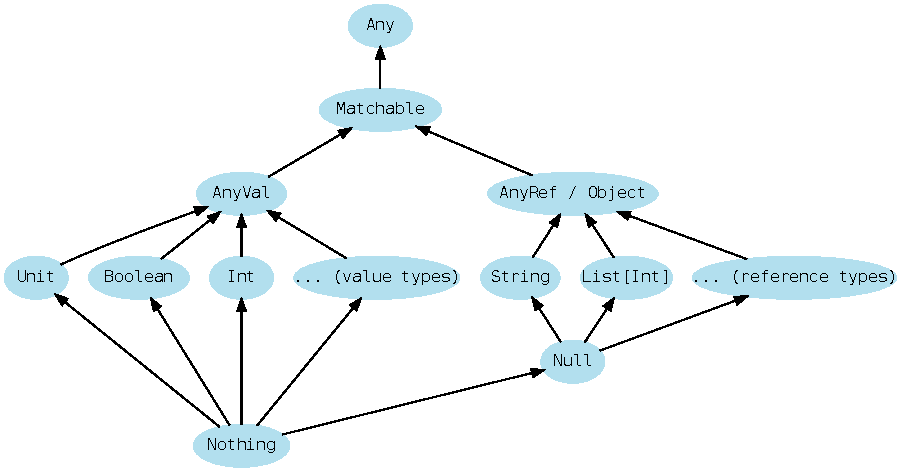
\includegraphics{images/type-hierarchy}
    \caption{Scala 3 type hierarchy.}
    \label{fig:scala-type-hierarchy}
\end{figure}

\todo{Pitäisikö varianssin olla irrallinen Scala-kappaleesta?}
Variance defines the rules on how the subtype relationship between parameterized types are dependent on the subtype relationship on the type on which it is parameterized. Variance has three variants: \textit{invariance}, \textit{covariance}, and \textit{contravariance}. Invariance means that subtyping relationships present in type parameters are not applied to the parameterized type at all. Covariance states that the subtype relationship of the parameterized type are in the same direction as a type parameter's subtype relationship. Contravariance means that the subtype relationship between parameterized types are the opposite way compared to the subtype relationships of the type parameter. A parametric type with multiple type parameters could declare each type parameter with different variance, for example functions in Scala are contravariant in their input type(s) and covariant in their result type. When \inlinecode{Sub} is a subtype of \inlinecode{Super} and \inlinescala{F[_]} is any parameterized type, then
\begin{itemize}
    \item Under covariance, \inlinescala{F[Sub]} is a subtype of \inlinescala{F[Super]};
    \item Under contravariance, \inlinescala{F[Super]} is a subtype of \inlinescala{F[Sub]}; and
    \item Under invariance, \inlinescala{F[Sub]} and \inlinescala{F[Super]} have no subtyping relationship.
\end{itemize}

Covariance is applicable in parameterized types that contain, store, or produce values, in other words the type parameter is in covariant position. Contravariance is applicable in the opposite situation, where values of the type parameter are consumed, i.e. the type parameter appears in a function parameter list, and is said to be in contravariant position. Invariance is useful in situations where it does not make sense for the parameterized type to have inheritance based on type parameter, or when the parameterized type is a mutable, or the type parameter appears both in covariant and contravariant positions.

An infamous example of mutable covariant type is primitive array in Java and C\# that perform a runtime type check when adding elements to the array, and throw exception if the type of the element is not compatible with the array, as demonstrated in \refsource{mutable-covariance}.
To avoid similar situation, mutable collections in Scala are invariant. Immutable collections and containers, such as \inlinecode{Option} or \inlinecode{Either} are covariant in Scala.

\begin{algorithm}

\begin{minted}{java}
String[] a = new String[1];	
Object[] b = a; // String is a subtype of Object, so this is legal
b[0] = 1; // Runtime exception since cannot add Integer to String[]
\end{minted}

\caption{Covariance in mutable types, like Java primitive array, is problematic \label{mutable-covariance}}
\end{algorithm}

Programming languages differ in the way the variance is defined. Languages like C\# and Scala define the variance with the parameterized type. In the other hand, language like Java define the variance only when using the parameterized type. The former is called \textit{declaration-site} variance, demonstrated in \refsource{declaration-site-variance} and the latter is called \textit{use-site} variance, demonstrated in \refsource{use-site-variance}. Approaches deviating from these exist, for example TypeScript tries to infer the variance, but has optional declaration-site annotations from version 4.7 onwards. Kotlin has declaration-site variance by default but emulates some parts of use-site variance with type projections. Invariance is the default in Scala and does not require explicit denotation. Covariance is declared with a \inlinecode{+} sign before each type parameter. Since contravariance could be seen as the opposite of covariance, it is denoted with a \inlinecode{-} sign.

\begin{algorithm}

\begin{minted}{scala}
class Invariant[A]      // Invariance is the default
class Covariant[+A]     // Covariance denoted with +
class Contravariant[-A] // Contravariance denoted with -
\end{minted}

\caption{Scala uses declaration-site variance, where the variance of a parameterized type is denoted in its type definition  \label{declaration-site-variance}}
\end{algorithm}

\begin{algorithm}

\begin{minted}{java}
interface Supertype {}
interface Subtype extends Supertype {}

void invariant(List<Supertype> list) {
    /* Get and set list values */
}
void covariant(List<? extends Supertype> list) {
    /* Only get list values */
}
void contravariant(List<? super Subtype> list) {
    /* Only set list values */
}
\end{minted}

\caption{Java has use-site variance, where the desired variance is declared when using the parameterized type \label{use-site-variance}}
\end{algorithm}

Many features and principles from functional programming are not only available, but also encouraged in Scala. Pattern matching, first-class functions (\refsource{scala:lambdas}), and tail recursion are all supported and heavily utilized in idiomatic Scala programs. Immutable variables, collections and data-structures are default the default way of writing Scala, even though mutable counterparts are also available. Functional data modeling is achieved with the use algebraic data types built into the language. Even though Scala embraces functional programming and imperative code is generally discouraged, introducing arbitrary side effects is possible.

\begin{algorithm}
\begin{minted}{scala}
val ns = List(1, 2, 3)

val mapped1 = ns.map(n => n + 1)
val mapped2 = ns.map(_ + 1) // Same as above in shorter form

val sum1 = ns.foldLeft(0)((x, y) => x + y)
val sum2 = ns.foldLeft(0)(_ + _) // Same as above in shorter form
\end{minted}

\caption{Long and short form of anonymous functions in Scala. \label{scala:lambdas}}
\end{algorithm}

In addition to ordinary functions, Scala has specific function called \inlinecode{PartialFunction} that is not defined for all values of its input type. It is a subtype of normal function and adds method \inlinecode{isDefinedAt}, which must be used to check before every function call whether the function is defined for the given value. Usually partial functions are not called directly by the programmer, but rather they are utilized in libraries to create better APIs. Partial functions are useful in pattern matching and many collection operators, such as \inlinecode{collect}, present in all standard library collections, which could be used instead of sequential \inlinecode{map} and \inlinecode{filter} operations. \refsource{scala:partial-function} shows how to define and use partial functions.

\begin{algorithm}
\begin{minted}{scala}
val someEvensMultipliedByTen: PartialFunction[Option[Int], Int] = {
  case Some(n) if n % 2 == 0 => n * 10
}

val opts  = List(None, Some(2), None, Some(3), Some(4))
val somes = opts.collect(someEvensMultiplied) // List(20, 40)
\end{minted}

\caption{Partial functions in Scala. \label{scala:partial-function}}
\end{algorithm}

Some functional languages, such as Haskell, have a special syntax for monadic computations. Scala also provides this syntactic sugar in a form of \inlinecode{for} comprehensions, demonstrated in \refsource{monad:for-syntax}. For comprehension is compatible with any data type that has \inlinecode{map} and \inlinecode{flatMap} methods defnied, such as \inlinecode{Option}, \inlinecode{Either}, and \inlinecode{ZIO} (chapter \ref{zio}). One could also add required methods to any type by using extension methods.

Being a academic language, Scala also has quite a lot more advanced features. Starting from extension methods, which enable to add methods to a class separately from its definition, operator overloading and infix operator- and method syntax, all the way to higher kinded and dependent types, type lambdas, as well as powerful meta programming capabilities. Scala 3 introduced more advanced features such as automatic type class derivation and union and intersections types.

Probably the most distinguishing feature in Scala is its implicit system and other contextual abstractions arising from that. Function could mark some of its parameters as implicit and the compiler would try to find that paramater from the enclosing scope by its type without programmer explicitly passing it as a parameter. Originally implicit parameters were introduced to achieve similar behavior as Haskell's type classes. Implicits could also be used for other purposes such as implicit conversions, context propagation, extension methods, and proving subtyping relationships between generic type parameters at compile-time.~\cite{tc-as-objects}

Function can mark some of its parameters as implicit with the keyword \inlinecode{using}. When the function is called, the compiler tries to find a value marked as implicit, with the keyword \inlinecode{given}, from the enclosing scope. If all requested values are found, they automatically inserted as parameters. If any of the implicit parameters is not found, an compilation error is reported. \refsource{scala:implicits} demonstrates function \inlinecode{summon}, which simply searches for implicit value by type, and the definition and usage of implicit parameters.

\begin{algorithm}
\begin{minted}{scala}
case class Person(age: Int, name: String)

// Define type class
trait Show[A]:
  extension (a: A) def show: String

// Define type class instance
given Show[Person] with
  extension (a: Person)
    def show: String = s"${a.name} is ${a.age} years old"

// Use the type class
def showAll[A: Show](as: List[A]): List[String] =
  as.map(a => a.show)
\end{minted}

\caption{Implicits could be used to encode type classes \label{scala:typeclasses}}
\end{algorithm}

Another advanced feature utilizing implicit resolution, is the ability of the Scala compiler to prove type equality or sub type relationships. There are two classes \inlinescala{=:=[From, To]} for type equality and \inlinescala{<:<[From, To]} for sub type relationship. Both classes extend a function \inlinescala{From => To}, and can be used to transform types. Types with two type parameters could be used as infix in Scala, for example type equality could be written \inlinescala{A =:= B}. When requesting implicit parameter of either of the types above, Scala compiler synthesizes an instance if the type relationship holds, otherwise reports a compilation error. The act of proving type relationships is said to be \textit{witnessing}, and a common practice is to name the implicit parameter as \textit{evidence}. The feature is useful, for example, when defining functions that make sense only for specific types, as demonstrated in \refsource{scala:witness}, where only nested \inlinecode{Maybe} types could only be flattened.

\begin{algorithm}
\begin{minted}{scala}
enum Maybe[+A]:
  case Just(a: A)
  case Nothing

  def flatten[B](using evidence: A <:< Maybe[B]): Maybe[B] =
    this match
      case Just(a) => evidence(a)
      case Nothing => Nothing

Maybe.Just(Maybe.Just(1)).flatten // Compiles
Maybe.Just(1).flatten // Error: Cannot prove that Int <:< Maybe[B]
\end{minted}

\caption{Scala compiler can prove (witness) a subtype relationship by providing implicit evidence. \label{scala:witness}}
\end{algorithm}

Another thing that sets Scala 2 and 3 apart is the introduction of intersection and union types in Scala 3. Intersection types are denoted with \inlinecode{&} symbol and union types with \inlinecode{|}. Intersection \inlinescala{A & B} means that the resulting type has properties of both \inlinecode{A} \textbf{and} \inlinecode{B}. Union is the dual of intersection, and the resulting type of \inlinescala{A | B} is either \inlinecode{A} \textbf{or} \inlinecode{B}.

Intersection types are commutative, idempotent, and have \inlinecode{Any} as the identity element. Commutativity means that the order of types included in the intersection does not matter, and Scala considers permutations equal. Idempotency states that type in intersection with itself is equal to the type itself. \inlinecode{Any} as the identity element means that the intersection of any type \inlinecode{A} with \inlinecode{Any} is equal to \inlinecode{A}, since all types themselves are subtypes of \inlinecode{Any}. Laws of intersection types witnessed by the Scala compiler:
\begin{itemize}
    \item Commutativity: \inlinescala{summon[(A & B) =:= (B & A)]}
    \item Idempotency: \inlinescala{summon[A =:= (A & A)]}
    \item Identity: \inlinescala{summon[A =:= (A & Any)]}
\end{itemize}

Like intersection types, also union types are commutative, idempotent, and have \inlinecode{Nothing} as the identity element. \inlinecode{Nothing} as the identity element means that the union of any type \inlinecode{A} with \inlinecode{Nothing} is equal to \inlinecode{A}, since there is no values of type \inlinecode{Nothing}. Laws of union types witnessed by the Scala compiler:
\begin{itemize}
    \item Commutativity: \inlinescala{summon[(A | B) =:= (B | A)]}
    \item Idempotency: \inlinescala{summon[A =:= (A | A)]}
    \item Identity: \inlinescala{summon[A =:= (A | Nothing)]}
\end{itemize}


\subsection{Capture checking}
Scala 3 is based on a research language called Dotty. The name Dotty comes from \acronym{DOT}{Dependent object types}, which is the theoretical foundation behind Scala 3~\cite{essence-of-dot}. While writing the thesis, feature called Capture checking~\cite{capture-checking} was added to Dotty and later to Scala 3 as an experimental feature. The idea of capture checking is to enable effectful programming in direct style (discussed in section \ref{background:monad:syntax}), while tracking effects in the type system and providing strong static guarantees of the correctness of the program.

\textcite{scoped-capabilities} published a paper that describes their findings regarding modeling polymorphic effects with capabilities. The initial version of capture checking is based on their work. \todo{Onko viittaus järkevä?} In the paper, they criticize the currently widely used ways of managing effects, such as Java checked exceptions and monads, as lacking in both usability and flexibility, that result in complex and duplicated code. They conclude that this is due to the transitive nature of effects in function call chains, combined with the classical type-systematic approach that \textquote{characterize the shape of values but not their free variables}, and suggest that modeling effects with capabilities may circumvent the problems they described.

The goal of capture checking is to address many of the limitations in effectful programming. These include how to solve the "What color is your function" problem~\cite{what-color-is-your-function}, how to express effect polymorphism, how to combine manual and automatic memory management, how to express high-level concurrency and parallelism safely, and how to migrate already existing programs to this new style~\cite{odersky-twitter-caprese}. The research focuses on the usability aspect of static effect tracking, which likely will evolve around effect polymorphism, inferring the the captured capabilities, direct style of programming, and in general minimizing the overall syntactic overhead.

Capture checking aims to address effects such as throwing exceptions, IO, mutability, and suspending computations and continuations. Resources are similar to effects but have some distinct properties. Resources, such as file handles, network connections, or memory) must be acquired before use, and disposed afterward to possibly clean up to free up OS level resources. This leads to the observation that a resource has \textit{lifetime} in which it could be used, and the usage of already disposed resource should be prevented. For the same reason, the sharing of resource between multiple parties requires rules. The lifetime and rules should preferably be enforced statically by the type system. This is closely related to lifetimes in Rust~\cite{rust-lifetimes} and linear type systems in general.

The fundamental idea of capture checking differs from the traditional effect system approach. Common approach with effect systems is that it annotates the effects what the execution of an expression might have. Capture checking, in the other hand, keeps track of the captured free variables in expressions. This means that capability is a normal value, like any other variable in a program, and both resources and effects could similarly be modeled in this way. In the context of capture checking, an expression is pure if it does not capture, i.e. close over, any capability. To make programming with capabilities easier, the capabilities could be implicitly passed to expressions, instead of requiring to explicitly thread capabilities through a program. The implicit system in Scala should be well suited for this task.

Capture checking can be enabled in Scala version 3.2.1 onwards with the compiler option \inlinecode{-Ycc}. Annotation \inlinescala{@capability} is used to mark a class/trait as capability that could be tracked. Captured capabilities are annotated before type annotation inside braces, e.g.: \inlinescala{val a: {capability} Int = 1}. \refsource{scala:cc-eff-polymorphism} provides a larger example by defining a effect polymorphic \inlinecode{List.map} function and demonstrating its usage. The syntax of capture checking is highly experimental and may be subject to change in the future.

\begin{algorithm}
\begin{minted}{scala}
// Compiles with dotty 3.2.0-RC1-bin-SNAPSHOT

// '{f}' Means that mapCC captures all capabilities of function 'f'
// This makes mapCC effect polymorphic since the resulting
// capabilities are solely determined by capabilities of 'f'
extension [A](xs: List[A])
  def mapCC[B](f: A => B): {f} List[B] =
    xs match
      case hd :: tl => f(hd) :: tl.mapCC(f)
      case Nil     => Nil

// Class is marked as capability by annotating it
@annotation.capability class Console:
  def printLine(x: Any): Unit = println(x)

// Required capabilites are declaired as constructor parameters
class Example(using val cn: Console):
  val numbers: List[Int] = List(1, 2, 3)
  
  // When function passed to mapCC does not capture capabilities
  // the resulting value does not capture anything
  val doubled: List[Int] = numbers.mapCC(n => n * 2)

  // Here the function passed to mapCC captures console capability
  // thus the resulting value captures the same capability
  // indicated in the type as '{console}'
  val printed: {console} List[Int] = numbers.mapCC { n =>
    console.printLine(n)
    n * 2
  }
\end{minted}

\caption{Effect polymorphism with capture checking %
\label{scala:cc-eff-polymorphism}}
\end{algorithm}


Odersky and the research group received a grant for seven researchers over five years, starting in September 2022~\cite{capture-checking-grant}. The research project is called Caprese (Capabilities for resources and effects), that will focus on universal theory of resources and effects based on capabilities. It will be interesting to see the results of the research group in the coming years.  The direction in which the research will develop remains to be seen.



\section{Type classes}
Type classes are a way to achieve ad-hoc polymorphism. They were first introduced by \textcite{ad-hoc-less-ad-hoc} in 1989 as a way to enable operator overloading in a programming language with Hindley-Milner type system. Eventually type classes were implemented in Haskell, largely based on Wadler's and Blott's proposal. A couple of years later, when applications of monads and related algebraic structures in programming were discovered~\cite{comp-lambda-monads}, type classes were a natural way to implement such algebraic structures.

Type class is an abstraction that defines behavior to some generic type. This enables one to implement highly generic functions that works with any type that is constrained to belong to type class. A type is said to be part of a type class if it has \textit{instance} of that type class. Instance of a type class contains functions and/or values that implement the behavior of the type class. Instances are defined separately from the type which for the instance is for, thus allowing to provide type class instances for third party data types if so desired. Example in \refsource{typeclass} demonstrates how type classes enable to implement polymorphic functions that work with any data type that belongs to specific type class.

\begin{algorithm}
\begin{minted}{scala}
case class Money(amount: Int)

trait Ordering[A]:
  extension (lhs: A) def <(rhs: A): Boolean

given Ordering[Money] with
  extension (self: Money) def <(that: Money): Boolean =
    self.amount < that.amount

// Compatible with any data type that has instance for Ordering
def sort[A: Ordering](as: List[A]): List[A] = as.sortWith(_ < _)

val sorted = sort(List(Money(3), Money(1), Money(2)))
\end{minted}

\caption{Definition, implementation and usage of the Ordering type class in Scala.%
\label{typeclass}}
\end{algorithm}


\section{Monads} \label{background:monads}
Of particular interest in this thesis is the algebraic structure monad. Algebraic structures are a concept that define functions that operate on some parametric type, or types, and are governed by algebraic laws. Algebraic structures are often studied through the lense of category theory, a branch of theoretical mathematics that studies objects, transformations between objects and relationships between different categories. In this thesis algebraic structures and monads in particular are approached from the perspective of computer science, and focusing on how monads are capable of encoding effects.

Functor is a transformation between two categories. In functional programming most, if not all, functors are endofunctors which are transformations from one category back to the same category. In practice endofunctors wrap some other category and allow to transform the inner category while preserving the outer category. List datatype is example of an endofunctor, because it allows to apply transformations to elements in the list, resulting in a new list. Monad is a special kind of endofunctor that is capable of collapsing a nested endofunctor structure. In the case of list, this means that every element in the list is transformed to a list, but the resulting list is not list of lists, but the inner lists are flattened. Listings \ref{functor:haskell} and \ref{functor:scala} show the definition of Functor type class in Haskell and Scala.

\begin{algorithm}

\begin{minted}{haskell}
class Functor f where
  fmap :: (a -> b) -> f a -> f b
\end{minted}

\caption{Functor type class in Haskell. %
\label{functor:haskell}}
\end{algorithm}


\begin{algorithm}

\begin{minted}{scala}
trait Functor[F[_]]:
  extension [A](fa: F[A]) def map[B](f: A => B): F[B]
\end{minted}

\caption{Functor type class in Scala 3 %
\label{functor:scala}}
\end{algorithm}

The applicability of monads for computer science was not discovered until the late 80s by \textcite{comp-lambda-monads} who described how the monad could be useful for defining semantics of effectful program. Moggi's proposed semantics extends lambda calculus in a pure way to support calculations previously considered to be impure. Later the idea of using monads to describe effectual computations was refined by \textcite{comprehending-monads}, \textcite{notions-computations} and \textcite{monads-for-fp}.

Any data type can form a monad if it has at least two capabilities: lifting any value to the context of the monad (i.e., the data type), and sequentially composing computations that act on these values. Every computation in these sequences has access to the values that previous computations may have produced. These computations produce values that are inside a data type and succeeding computations have access to. Lifting and sequencing must adhere to monad laws in order for the data type to be considered a monad. Monad laws are discussed in more detail in section \ref{monad:laws}.

In practice several data types naturally form a monad, such as \inlinecode{Array} in JavaScript with \inlinecode{of} function providing lifting and \inlinecode{flatMap} function providing sequencing~\cite{js-array}. Monads and other algebraic structures are often implemented as typeclasses, and writing programs consists of operations provided by the typeclass. This allow for writing highly abstract programs where generic types are constrained by requiring them to be part of certain type class. Definition of monad type class in Haskell and Scala are provided in Listings \ref{monad:haskell} and \ref{monad:scala}.

\begin{algorithm}

\begin{minted}{haskell}
class Functor m => Monad m where
  return :: a -> m a
  ( >>= ) :: m a -> (a -> m b) -> m b
\end{minted}

\caption{Monad type class in Haskell. %
\label{monad:haskell}}
\end{algorithm}


\begin{algorithm}

\begin{minted}{scala}
trait Monad[F[_]]:
  def pure[A](a: A): F[A]
  extension [A](fa: F[A]) def flatMap[B](f: A => F[B]): F[B]
\end{minted}

\caption{Monad type class in Scala 3 %
\label{monad:scala}}
\end{algorithm}

Composing programs of sequential instructions is nothing new compared to imperative programming. Monads, however, can control what effects are possible within such computations. The data type (i.e. monad) provides the context in which the computations are performed, and thus defines the semantics of lifting and sequencing. Different monads have different semantics and that allows encoding different effects with monads. The usefulness of monads comes from the fact that sequencing computations one after the other is such a primitive operation in any effectful program. Monads abstract this fundamental operation, and allow to define the meaning of sequentiality in the context of a specific monad. For example in a list monad, the semantics of sequencing is to perform the computation for every element in the list, and composing multiple lists will result in a cartesian product, demonstrated in \refsource{monad:bind}. Examples of other monads and their semantics are introduced in more detail later in this chapter.

\begin{algorithm}

\begin{comment}
\begin{minted}{haskell}
name :: IO ()
name =
  putStrLn "What's your name?" >>= \_ ->
  getLine >>= \name -> 
  putStrLn ("Nice to meet you " ++ name)
\end{minted}
\end{comment}


\begin{minted}{haskell}
suits = ["Club", "Heart", "Diamond", "Spade"]
ranks = [2..14]

-- [("Club", 2), ("Club", 3), ... ,("Spade", 13), ("Spade", 14)]
deck =
  suits >>= \suit ->
  ranks >>= \rank ->
  return (suit, rank)
\end{minted}

\caption{Monadic bind in list monad results in a cartesian product %
\label{monad:bind}}
\end{algorithm}

Even though the naming of the lifting and sequencing functions does not determine whether data type forms a monad or not, knowing some of the most common naming conventions is beneficial, even though naming of these functions varies and is dependent on the programming language, library and framework. The lifting function is usually called \inlinecode{pure}, \inlinecode{return}, \inlinecode{unit}, or \inlinecode{succeed}, and the sequencing function is called \inlinecode{bind}, \inlinecode{flatMap}, \inlinecode{chain}, or symbolic alias \inlinecode{>>=}.

In addition to these mandatory functions, monads commonly define more specific functions that only make sense in the context of a particular monad. These functions make it easier and more convenient to use the capabilities of the monad, or possibly to change the behavior of computations in some way. Examples of such functions are presented along with the introduction of specific monad types

Monads are traditionally associated with statically typed languages, although there is nothing to prevent their use in a dynamically typed language. In statically typed languages monads naturally work as an effect system by making it explicit in the type system if and what effects are involved. When mixing multiple effects with each other, type signatures can get quite chaotic. We will get back into this subject when discussing about monad transformers.


\subsection{Id}
A trivial example of a monad is the identity or \inlinecode{Id} monad. It simply encodes the effect of having no effect at all. Lifting values to monadic context is trivial since no lifting is required. The semantics of sequencing does not differ from conventional function application, as demonstrated in \refsource{monad:id}.

\begin{algorithm}

\begin{minted}{scala}
type Id[A] = A
      
given Monad[Id] with
  def pure[A](a: A): Id[A] = a
  extension [A](a: Id[A])
    def flatMap[B](f: A => Id[B]): Id[B] = f(a)
\end{minted}

\caption{Identity monad in Scala. %
\label{monad:id}}
\end{algorithm}


\subsection{Either} \label{background:monads:either}
\inlinecode{Either} monad encodes the effect of raising and handling exceptions when performing computations that might fail. Since \inlinecode{Either} is a monad, it enables the sequential composition of multiple possibly failing computations. Like the name suggest, computations in \inlinecode{Either} monads can either succeed with value or fail with an exception. Either has similar short-circuiting semantics as throwing exceptions in, e.g. Java. When the first exception is encountered, succeeding computations will not be performed and the exception remains as the result of the computation. Usually \inlinecode{Either} provides combinators that can transform a failed computation into a successful one. This is semantically similar to catching exceptions. Unlike throwing and catching exceptions, \inlinecode{Either} makes it obvious in the type signature of the function that the computation the function describes has a possibility of failure.

\begin{algorithm}

\begin{minted}{scala}
enum Either[+E, +A]:
  case Left(e: E)
  case Right(a: A)

given [E]: Monad[[A] =>> Either[E, A]] = new:
  def pure[A](a: A): Either[E, A] = Right(a)

  extension [A](either: Either[E, A])
    def flatMap[B](f: A => Either[E, B]): Either[E, B] =
      either match
        case Left(e)  => Left(e)
        case Right(a) => f(a)
\end{minted}

\caption{Either monad in Scala. %
\label{monad:either}}
\end{algorithm}

In practice the \inlinecode{Either} data type is commonly implemented as a sum type of two variations: \inlinecode{Left} (exception) and \inlinecode{Right} (success). Usually implementations are right-biased which, among other things, determines the semantics of monadic operations. To lift a value into \inlinecode{Either} monad, the value is simply wrapped in \inlinecode{Right}. The meaning of sequencing in the case of \inlinecode{Right} is to pass successful value to subsequent computations, whereas in the case of \inlinecode{Left} it is returned as is and no computations are performed. An example of implementation in Scala is given in \refsource{monad:either}

In order for \inlinecode{Either} to better support exception handling, several convenience functions are commonly defined for it. These functions are more specific than the monad structure admits, since they operate in a domain where the computation might produce different values. Next a few of the these functions are introduced in more detail.

One typical scenario in error handling is to define a fallback computation to be performed if the actual computation is unsuccessful. In Haskell this is achieved by utilizing a associative binary operation in \inlinecode{Semigroup} typeclass, which is defined as \inlinehaskell{(<>) :: Either e a -> Either e a -> Either e a}. In Scala similar semantics is made possible by \inlinecode{orElse} -method on an \inlinecode{Either} object itself defined as \inlinescala{def orElse[E1, A1](or: => Either[E1, A1]): Either[E1, A | A1]}. Because Scala 3 has union and subtypes, it is possible for the fallback computation to have different exception and success types as the original \inlinecode{Either}.

Another common operation in error handling is to transform the error type. There are some differences in the implementation of this functionality depending on the language. Haskell has \inlinecode{BiFunctor} typeclass where the function \inlinecode{first} allows to apply transformations to the left side of either. Scala has \inlinecode{LeftProjection}, which allows to perform monadic operations on the (left) error "channel" of the \inlinecode{Either}. \inlinecode{Either} in Scala also has \inlinescala{def swap: Either[A, E]} method that transforms a \inlinecode{Right} to \inlinecode{Left} and vice versa.

Possibly the most common operation in error handling is to derive some final value from a computation. Since the computation could have either failed or succeeded, both possibilities must be covered. This could be achieved by providing a function for both cases that transforms the corresponding value (failure or success) to the same result type. In Haskell the function is \\\inlinehaskell{either :: (a -> c) -> (b -> c) -> Either a b -> c} and in Scala it's \\\inlinescala{def fold[B](onLeft: E => B, onRight: A => B): B}. \todo{Tarkasta rivitys}

There is a similar monad to \inlinecode{Either} commonly called \inlinecode{Maybe} or \inlinecode{Option}. Like \inlinecode{Either} it has two variants: one that holds value of successful computation, and another that implies failure, but does not carry any useful information. Like mentioned in section \ref{effects:exceptions}, it is possible to encode the concept of optionality with exceptions. In cases when \inlinecode{Either}'s error type contains only a single value, it is isomorphic\footnote{Two types are isomorphic if it's possible to define a lossless transformation between them.} to \inlinecode{Option}. Example of this isomorphism in Scala is given in \refsource{isomorphism}. Both Haskell and Scala have the type \inlinecode{Unit} or \inlinecode{()} that has cardinality of one.

\begin{algorithm}

\begin{minted}{scala}
def optionToEither[A]: Option[A] => Either[Unit, A] = {
  case None    => Left(())
  case Some(a) => Right(a)
}

def eitherToOption[A]: Either[Unit, A] => Option[A] = {
  case Left(()) => None
  case Right(a) => Some(a)
}
\end{minted}

\caption{\inlinecode{Either} with \inlinecode{Unit} as error type is isomorphic to \inlinecode{Option}. %
\label{isomorphism}}
\end{algorithm}


\subsection{Reader}
The reader monad encodes the effect of describing a sequence of computations that require some shared context or environment in order to be evaluated. The idea closely resembles composing functions together by passing arguments from parent to child functions. Instead of explicitly passing every parameter, the reader monad automatically threads the environment through computations. It's noteworthy that the reader monad itself is nothing more than a data structure that describes a computation. In order to retrieve the described result the computation must be executed by providing the environment it requires. Common use-cases for reader monad are dependency injection and context sharing in deeply nested structures such as function calls or component hierarchies in UI frameworks.

\begin{algorithm}

\begin{minted}{scala}
case class Reader[-R, +A](run: R => A)

object Reader:
  def ask[R]: Reader[R, R] = Reader(r => r)

given [R]: Monad[[A] =>> Reader[R, A]] with
  def pure[A](a: A): Reader[R, A] = Reader(_ => a)
  extension [A](self: Reader[R, A])
    def flatMap[B](f: A => Reader[R, B]): Reader[R, B] =
      Reader(r => f(self.run(r)).run(r))
\end{minted}

\caption{Reader monad in Scala. %
\label{monad:reader}}
\end{algorithm}

The Implementation of the reader monad (\refsource{monad:reader}) is confusingly simple due to the fact that it's essentially just a wrapper for a function. It could be implemented as a single parameter function that receives the requirements as argument and returns the result of the computation. Lifting a value to a reader monad is as simple as defining a function that ignores it argument and returns specified value. The meaning of sequencing two reader computations together is to run both computations providing them with the same parameter.~\cite{fp-overloading-ho-polymorphism}.

Reader has a couple of common operations specific to it. One primitive operation is to retrieve the environment from the reader. The implementation is just an identity function, and the operation is often named \inlinecode{ask}, \inlinecode{get}, or \inlinecode{environment}. Another primitive operation is to actually run the computation the reader monad describes to get the final result from it. Running a reader monad is nothing more than providing the required environment, in some cases there is a helper function \inlinecode{run} or \inlinecode{runReader} to do just that.


\subsection{IO}
IO monad encodes the effect of performing side effects and possibly returning a value as a result of the side effect. This enables to implement programs that use, e.g., a console, file system, network or graphical user interface. It is common to also allow expressing mutability via IO monad. Also, modern IO monads usually provide a way to introduce as well as manage asynchrony, concurrency, and parallelism. With asynchronous operations comes the desire to define interruptions, timeouts and to handle asynchronous exceptions in a sound way, discussed in section \ref{effects:exceptions}.

Theoretical background of IO Monad is described by \textcite{imperative-fp}. This work was published a couple of years after Moggi's initial discovery of using monads to model effects. IO monad was originally designed for Haskell, which is a lazily evaluated and purely functional programming language. Due to being a lazy language, there is no explicit control flow and terms are evaluated only when absolutely required. Programming with side effects, however, requires that they are executed in a precisely defined order. Wadler and Peyton-Jones describes the relationship between lazy evaluation and side effects as follows: \textquote{laziness and side effects are fundamentally inimical}. Every expression in Haskell must be referentially transparent and programming with side effects is no exception. Modeling side effects with monads retains referential transparency and determines the execution order of expressions.

Wadler and Peyton-Jones describe a parametric data type \inlinehaskell{IO a} that represents a possibly side effecting program that, \textbf{when executed}, returns a value of type \inlinecode{a}. In other words, \inlinehaskell{IO a} is an ordinary value that can be transformed by passing it into functions that return modified IO values. Also, a program may choose not to execute certain IO values even though they are defined. This idea of modeling side effecting programs as values turned out to be highly useful. It provides superior composability compared to programs with unrestricted side effects. For example it is possible to define combinators that work with every IO program and thus define behaviors like retrying, timeouts, error handling, parallelism and racing in a reusable manner.

IO monads and the idea of programs as values has been adopted to other languages than Haskell as well, including many impure and eagerly evaluated. Examples of such implementations are \titlecite{zio}, \titlecite{cats-effect} and \titlecite{monix} in Scala, \titlecite{effect-ts} in JavaScript/TypeScript, \titlecite{arrow-fx} in Kotlin, \titlecite{missionary} in Clojure, and \titlecite{purescript-eff} and \titlecite{purescript-aff} in PureScript.
% \begin{itemize}
%     \item Haskell IO
%     \item Haskell RIO (https://www.fpcomplete.com/haskell/library/rio/)
%     \item Rust Tokio ?
% \end{itemize}

Lifting a value into the IO monad means that no side effects are performed and the value is simply wrapped to IO. This bridges the cap between pure and impure worlds by making it possible to bring pure values into a context where describing side effects is possible.
The meaning of sequencing is to create a description of two side effects that, when executed, are performed one after another. Like with all monads, the latter IO has access to the value produced by the preceding IO computation. A simple example implementation of IO monad is given in \refsource{monad:io}.

\begin{algorithm}

\begin{minted}{scala}
case class IO[A](run: () => A)

given Monad[IO] = new:
  def pure[A](a: A): IO[A] = IO(() => a)
  extension [A](io: IO[A])
    def flatMap[B](f: A => IO[B]): IO[B] =
      IO(() => f(io.run()).run())
\end{minted}

\caption{Naive IO monad in Scala %
\label{monad:io}}
\end{algorithm}

The IO monad is fundamentally different from previously introduced monads, which can be implemented in a referentially transparent way. Since the IO monad encodes side effects it is inherently not referentially transparent, because the side effects must be executed \textit{at some point}. To make it possible to write side-effecting programs in a purely functional way, the IO monad separates the description of side effects from the execution of side effects. Constructing a description of a side-effecting program is referentially transparent, while its execution is not, the latter is delayed, usually happening outside of "user-land" code.

To actually perform the side effects IO describes, there must be a way to interpret IO values into side effects they describe. This is usually the responsibility of the particular \textit{runtime system}. In a purely functional programming language, the runtime cannot be implemented in the language itself. Impure languages have more flexibility in the way of implementing the runtime system, as well as how to encode the IO monad in the first place. Modern runtime systems with industry adoption are enormously complex and sophisticated, to utilize the hardware as efficiently as possible to achieve the best performance possible.

Performance is really important, since the usa of IO monad in a program is intrusive.
Any expression that references another expression that is evaluated in IO, must also be evaluated in IO. This is to be expected as there is no way to "peel off" the IO wrapper from an expression in a referentially transparent way, since that would mean executing the side effect. \todo{Entä effect handlers, language level CPS-transformation (Kotlin, Scheme) tai monadic reflection ?}
The runtime system can be seen as the central authority in effectful programs, as described in section \ref{effects}.



\subsection{Syntax} \label{background:monad:syntax}
The "usual" kind of code where functions are applied to values is called \textit{direct style}. Programming with wrapped types (endofunctors), like monads, enforces a different style of syntax called \textit{monadic style}. To perform operations on values in the monadic context, like combining multiple values together, one must use higher-order combinators, such as \inlinecode{map} and \inlinecode{flatMap}. The sequencing combinator will bind the value inside the monad to a variable that could be used in a function. \refsource{monad:syntax} compares the direct style to monadic style, by the means of usual integer addition and integer addition in the Option monad.

\begin{algorithm}

\begin{minipage}{0.35\textwidth}
\begin{minted}{scala}
// Direct style
val num1: Int = 3
val num2: Int = 4
val sum: Int  =
    num1 + num2
    

\end{minted}
\end{minipage}
%
%\hspace{0.05\textwidth}
%
\begin{minipage}{0.45\textwidth}
%\vspace{0.05\textwidth}
\begin{minted}{scala}
// Monadic style
val optionNum1: Option[Int] = Option(3)
val optionNum2: Option[Int] = Option(4)
val optionSum: Option[Int]  =
  optionNum1.flatMap(n1 =>
    optionNum2.map(n2 =>
      n1 + n2))
\end{minted}
\end{minipage}
    
\caption{Direct vs. monadic syntax in Scala %
\label{monad:syntax}}
\end{algorithm}


Programming with monads leads to numerous sequencing functions one after another. This requires more typing, and the intent of the code might be harder to see because it is obfuscated by the "monadic machinery". Some languages have built-in support for representing monadic computations in a more convenient way. Usually this comes in the form of special syntax for sequencing multiple monadic computations together with minimum boilerplate. The syntax is nothing more than syntactic sugar that the compiler converts to calls to monadic sequencing functions. Examples of such syntax are \textcite{haskell-do-notation}, \textcite{scala-for-comprehension}, \textcite{fsharp-computation-expression}, and \textcite{ocaml-bind-ops}. \refsource{monad:for-syntax} compares Scala's for-comprehension syntax that desugars to sequence of \inlinecode{flatMap}s and one final \inlinecode{map} function.

\begin{algorithm}

\begin{minipage}{0.40\textwidth}
\begin{minted}{scala}
val optionSum: Option[Int] =
  optionNum1.flatMap(n1 =>
    optionNum2.map(n2 =>
      n1 + n2))
\end{minted}
\end{minipage}
%
\hspace{0.05\textwidth}
%
\begin{minipage}{0.40\textwidth}
%\vspace{0.08\textwidth}
\begin{minted}{scala}
val optionSumFor: Option[Int] = for
    n1 <- optionNum1
    n2 <- optionNum2
  yield n1 + n2
\end{minted}
\end{minipage}

\caption{For-comprehension in Scala %
\label{monad:for-syntax}}
\end{algorithm}


A technique for programming in direct style with monadic effects while preserving the semantics of the specific monad has been proposed~\cite{representing-monads}. The technique is called \textit{monadic reflection}, and it utilizes the fact that programs written in monadic style could be translated into programs written in \acronym{CPS}{Continuation Passing Style}. The proposed technique requires from the programming language or platform a language-level support for first-class continuations/suspensions/coroutines \todo{sopiva ilmaus?}. Monadic reflection requires for each monad an implementation of a type class with two operations: \inlinecode{reify} and \inlinecode{reflect}, that wrap and unwrap values to and from monadic context. The original idea was to have monadic effects in Scheme, but in practice monad reflection has hardly gained any traction in a functional library or language. There has been some recent research on how monadic reflection could work with capability-based effect tracking in Scala, and also a proof-of-concept implementation in Scala 3~\cite{representing-monads-capabilities, monadic-reflection-scala}.


\subsection{Monad Laws} \label{monad:laws}
For a data type to form a monad, it must adhere to three laws, also known as the monad laws: associativity, left identity, and right identity. These laws are simply rules that the operations on a data type must follow. The laws precisely define the semantics of a data type and allow to freely refactor programs and define combinators while preserving the desired semantics. Laws are what separate one algebraic structure from another. To be precise, algebraic structure is totally defined by its operations and the laws that govern these operations. Thus the definition of monad is an algebraic structure with two operations
\inlinecode{pure} and \inlinecode{bind}, obeying the laws of associativity, left identity, and right identity, nothing more, nothing less.~\cite{fp-in-scala}

\begin{algorithm}

    \begin{minted}{scala}
                def pure[A](a: A): Option[A] = Monad[Option].pure(a)
                
                val num1: Option[Int] = Some(1)
                val num2: Option[Int] = Some(2)
                val num3: Option[Int] = Some(3)
                
                val mustBeTrue = sumAll1 == sumAll2
    \end{minted}

    \begin{minipage}{0.40\textwidth}
    \begin{minted}{scala}
def sumAll1: Option[Int] = 
  num1.flatMap(n1 =>
    num2.flatMap(n2 =>
      num3.flatMap(n3 =>
        pure(n1 + n2 + n3))
    )
  )
    \end{minted}
    \end{minipage}
    %
    \hspace{0.05\textwidth}
    %
    \begin{minipage}{0.40\textwidth}
    \vspace{0.05\textwidth}
    \begin{minted}{scala}
    def sumAll2: Option[Int] =
      num1.flatMap(n1 =>
        num2.flatMap(n2 =>
          pure(n1 + n2))
      ).flatMap(sum12 =>
        num3.flatMap(n3 =>
          pure(sum12 + n3))
      )
    \end{minted}
    \end{minipage}

    \caption{Monad associativity law in Scala. %
    \label{monad:laws:associativity}}
\end{algorithm}

Associativity means that if there is a binary operation \footnote{Function that takes two values and produces another value} that is applied to three or more values, the order of application does not change the resulting value. In other words, the order of parentheses does not matter. Common examples of associative operations include integer addition and multiplication, string concatenation, and boolean \inlinecode{&&} and \inlinecode{||} operations. In the context of monads associativity states that the semantics of sequencing are not dependent on nesting of \inlinecode{bind} operations. Example of this is provided in \refsource{monad:laws:associativity}.

\begin{algorithm}

\begin{minted}{scala}
def pure[A](a: A): Option[A] = Monad[Option].pure(a)
def f(n: Int)                = pure(n + 1)

// Left identity
val x: Int = 1
pure(x).flatMap(n => f(n)) == f(x)

// Right identity
val num: Option[Int] = pure(1)
num.flatMap(n => pure(n)) == num
\end{minted}

\caption{Monad identity laws in Scala. %
\label{monad:laws:identity}}
\end{algorithm}

Left and right identity laws define how lifting and sequencing must interoperate. Left identity states that if a value is lifted to monadic context and then the value is applied to function using sequence, it must be equal to just applying the value to the function without lifting into monadic context. Right identity states that if a value is lifted into monadic context and sequenced into lifting function, it must be equal to original lifted value. Example of both identity laws is provided in \refsource{monad:laws:identity}.


\subsection{Monad transformers}\label{background:monad:monad-transformers}
So far we have gone through how monads can be used to encode several side effects. However in practice it is really common that multiple effects need to be used in tandem. Practically all applications use the IO monad, may desire to model exceptions and early termination with the Either monad, and access configuration or other context provided by the Reader monad. There is nothing to prevent manually stacking multiple monads to achieve all these functionalities.

Stacking multiple monads will lead to nested type signatures. The order of stacking is really important, as same types nested in different order may imply totally different meaning. \todo{i.e. stacking monads is not commutative} For example \inlinescala{IO[Either[Error, Success]]}, is a side effecting program that produces either a result of type \inlinecode{Success} or fails with an exception of type \inlinecode{Error}. In the other hand, expression of type \inlinescala{Either[Error, IO[Success]]} is a program that will in the success case perform some side effects to produce a value of type \inlinecode{Success}, or fail with exception of type \inlinecode{Error} without any side effects.

Also programming with nested monads leads to added boilerplate. To lift value in to a nested monad, it must be manually wrapped with every monad in the correct order.
The programmer must manually thread the value inside monad layers through the program while preserving the nesting order and semantics of each monad. Every monad has slightly different semantics, so implementation details differentiate depending on the monad type. \refsource{monadtransformer:io-either} demonstrates required syntax when programming with nested IO and Either monads.

\begin{algorithm}

\begin{minted}{scala}
def fn(str: String): IO[Either[Unit, Int]] = ???

val ioEitherString: IO[Either[Unit, String]] = IO(Right("initial str"))

val ioEitherInt: IO[Either[Unit, Int]] =
  ioEitherString.flatMap(either =>
    either.fold(
      error => IO(Left(error)),
      success => fn(success),
    )
  )
\end{minted}

\caption{Syntax overhead of nesting Either and IO monads. %
\label{monadtransformer:io-either}}
\end{algorithm}

In addition to obfuscating the intent, manually implementing all of this functionality is a burden to the programmer and a possible source of bugs. Sometimes the cause of bugs could be highly subtle, for example when using Either for error handling inside IO. Example of this is provided in \refsource{monadtransformer:subtle-bugs}. The programmer might be relying on the short-circuiting semantics of Either but when used inside the IO monad, the error is silently swallowed. It is even possible that the return type of \inlinecode{mightFail} was initially \inlinescala{IO[Unit]}, and it was later refactored to also include an error case. In this situation, the compiler also does not report an error since discarding values is allowed. As there is arbitrarily many ways to nest monads, the number of similar possible bugs is indefinite.

\begin{algorithm}

\begin{minted}{scala}
def mightFail: IO[Either[String, Unit]]   = ???
def willNotFail: IO[Either[Nothing, Int]] = ???

val program: IO[Either[String, Int]] =
  for
                       // Type of _ is Either[String, Unit]
    _   <- mightFail   // Even if line evaluates to Left[String]
    res <- willNotFail // ... this line will still be executed
  yield res
\end{minted}

\caption{Subtle bugs not causing early termination or compilation error %
\label{monadtransformer:subtle-bugs}}
\end{algorithm}

Nesting monads does also come with performance considerations. The memory consumption is higher because each nested monad consumes some amount of memory. Also when calling monadic functions, the calls must propagate through every layer of nesting, thus increasing indirection by raising the number of function calls. The exact magnitude of performance implications depends on the  language, platform, and runtime environment. Haskell runtime is quite efficient with this style of code, while the JVM is not. \todo{Tarvisiko tähän lähteen väitteiden tueksi?}

\begin{algorithm}

\begin{minted}{scala}
case class EitherT[F[_], E, A](effect: F[Either[E, A]])

given [E, F[_]: Monad]: Monad[[A] =>> EitherT[F, E, A]] = new:
  def pure[A](a: A): EitherT[F, E, A] =
    EitherT(Monad[F].pure(Right(a)))

  extension [A](self: EitherT[F, E, A])
    def flatMap[B](f: A => EitherT[F, E, B]): EitherT[F, E, B] =
      EitherT(
        self.f.flatMap {
          case Left(e)  => Monad[F].pure(Left(e))
          case Right(a) => f(a).f
        }
      )
\end{minted}

\caption{EitherT monad transformer in Scala. %
\label{monadtransformer:either-t}}
\end{algorithm}

For this purpose there is a concept called monad transformers that allows to compose multiple monads into one. There is not a universal way to compose monads this way. Because of this, each monad must have its own monad transformer instance. For some monads it is not possible at all to define a monad transformer. Monad transformer is simply just a wrapper for some monad that has semantics of both monads, just like nested monads. Like every monad, the composed monad must obey to monad laws.

The nested monad in \refsource{monadtransformer:io-either}, \inlinescala{IO[Either[E, A]]}, is isomorphic to \inlinescala{EitherT[IO, E, A]} (defined in \refsource{monadtransformer:either-t}) which is a monad transformer for Either monad applied to IO. This monad is capable of encoding side effects as well as terminating early in the presence of errors. \refsource{monadtransformer:either-t-io} demonstrates identical program as in \refsource{monadtransformer:subtle-bugs} but it does not suffer from issues described earlier since EitherT composes any other monad with short-circuiting semantics.

\begin{algorithm}

\begin{minted}{scala}
def mayFail: EitherT[IO, String, Unit]  = ???
def wontFail: EitherT[IO, Nothing, Int] = ???

val program: EitherT[IO, String, Int] =
  for
                      // Type of _ is Unit
    _     <- mayFail  // If this line produces error
    value <- wontFail // This line won't be executed
  yield value
\end{minted}

\caption{Usage of EitherT monad transformer with IO monad.%
\label{monadtransformer:either-t-io}}
\end{algorithm}

Monad transformers alleviate some of the issues encountered when nesting monads manually. There is less syntactic overhead since the monad transformer threads the values through the monad stack and does all required wrapping and unwrapping. However, many of the problems with nested monads are also present in monad transformers. The order of nesting is still significant, performance considerations are similar and every monad requires unique implementation. 

Because Scala has subtyping, it emposes some unique constraints to monad transformers. EitherT defined in \refsource{monadtransformer:either-t} was invariant on the monad it composes. With this definition the code in \refsource{monadtransformer:either-t-io} will not compile since \inlinecode{mightFail} and \inlinecode{willNotFail} do not have identical type signatures. To overcome this issue, there exists multiple solutions each with their pros and cons. One might define the EitherT to require the composed monad to be covariant. This has the obvious downside that it restricts what monads are compatible with EitherT. Other option would be to define widening operators on invariant EitherT, but that would place a burden on the programmer who would have to explicitly invoke those methods. Both options are demonstrated in \refsource{monadtransformer:either-t-variance}.

\begin{algorithm}

\begin{minted}{scala}
case class CovariantEitherT[F[+_], +E, +A](effect: F[Either[E, A]])

case class EitherT[F[_], E, A](effect: F[Either[E, A]]):
  def leftWiden[E1 >: E]: EitherT[F, E1, A] =
    this.asInstanceOf[EitherT[F, E1, A]]
\end{minted}

\caption{EitherT leftWiden method %
\label{monadtransformer:either-t-variance}}
\end{algorithm}

\todo{Pitäisikö mainita jotain monadeista ja effect polymorfismista?}

% -----------------------------------------------------------------------------------------------------
% -----------------------------------------------------------------------------------------------------
% -----------------------------------------------------------------------------------------------------
\section{Algebraic effects and handlers} \label{background:alg-eff}
Algebraic effects and handlers is one of the most recent approach and field of research on the subject of purely functional effectful programming. Algebraic effects take the approach that there are variety of different types of effects and every effect type has a finite set of \textit{operations} which define potentially impure capabilities. To interpret each operation, one must provide \textit{handler} for every effectful operation. Operations define the interface of the effect, while handlers define the semantics of each effect and operation.

The notion of \textquote{algebraic operations} was introduced by \textcite{adequacy-for-alg-effs} in \citeyear{adequacy-for-alg-effs} and they refined the idea in \cite{comp-effs-and-ops} and \cite{alg-ops-gen-effs}. The idea of handlers accompanying algebraic effects was first presented by \textcite{handlers-of-alg-effs} in \citeyear{handlers-of-alg-effs} and later \textcite{handling-alg-effs} in \citeyear{handling-alg-effs}. The idea was similar to what Moggi discovered in \cite{notions-computations}, but \citeauthor{adequacy-for-alg-effs} considered operations to be primitive instead being derived from the monadic context. \todo{Mitä tämä tarkoittaa?}

The applicability of algebraic effects and handlers is mostly, at least currently, in strict/eagerly evaluated purely functional programming languages. The idea of transferring the control to an effect handler does not fit the model of lazily evaluated languages naturally, since lazy evaluation does not have explicit control flow in the first place.~\cite{alg-effs-for-fp}

% -----------------------------------------------------------------------------------------------------
\subsection{Existing languages and libraries}
Algebraic effects could be implemented as a library or a language-level feature. There exists several libraries aiming to add support for algebraic effects in languages that do not have native support for them like Idris Effects~\cite{idris-effects}, Haskell Extensible effects~\cite{extensible-effects} and F\# AlgEff~\cite{fsharp-alg-eff}. In the 2010s the theory of algebraic effects evolved in to several research languages such as Eff~\cite{eff-lang}, Koka~\cite{koka-lang}, Frank~\cite{frank-lang}, Links~\cite{links-lang}, and Effekt~\cite{effekt-lang}. The first appearances of algebraic effects in non-research languages have happened in the recent years with Unison~\cite{unison-lang} and OCaml~\cite{ocaml-lang}.

Unison is a programming language with several out-of-the-ordinary features including \textit{abilities}, which are an implementation of algebraic effects from Frank~\cite{frank-lang}. OCaml version 5.0 includes~\cite{ocaml-mc-sep-2021} language-level support for algebraic effects. Unison have had alpha and beta versions since 2019 and is currently aiming to achieve commercial adoption. OCaml 5.0 is in alpha as of September 2022 and stable version planned to be released in the near future. As can be seen, currently algebraic effects are a new concept with little to none industry experience.

% -----------------------------------------------------------------------------------------------------
\subsection{Theory of handlers}
When program encounters an effect operation, its execution is halted, and the control is transferred to the closest handler provided for that specific operation. Handler may also receive some parameters from the program, in the process of taking over the execution from the program. At this point, it is solely the responsibility of the handler to decide how the program will continue.

The idea of effects being interaction between sub-programs and central authority, described in section \ref{effects}, fits algebraic effects naturally. Parts of the program calling effect operations are the sub-program and handlers are the central authority. The concept is powerful enough to implement all previously mentioned monads and even many of the more complicated control structures, built-in to many languages, like try-catch, iterators, and async/await.~\cite{alg-effs-for-fp} \todo{Mainitse myös backtracking ?}

\todo{Sopiiko seuraava kappale tähän? Pitäisikö siirtää conclusoneihin?}
Algebraic effects offer a referentially transparent way to model effects, as programs are implemented to work with the effect interface, and actual effects are performed by the handlers. The concept of separating the definition of effects from the semantics, i.e. interpretation or implementation, and giving handlers the full power to specify how the program will continue, enables implementation of truly expressive and elegant abstractions.

Common way of implementing handlers is to transform the effect to another effect or data type. Many times higher-level effects are implemented in terms of lower level effects, and finally the most primitive effects, such as IO, are provided by runtime. Eventually this forms a graph of effects and handlers depending on each other.~\cite{intro-to-alg-eff} Providing an expression with a effect handler it requires is said to \textquote{discharge} the effect from the expression. In order to successfully execute a program all of its effects must be discharged.

Handlers have a way to continue executing the program, and optionally apply a transformation function to the final value of the expression they handle. However it is totally up to the specific handler to decide how and if to continue the execution or whether to apply the final transformation. This way the handler full power to decide how to act. It may continue the execution and, depending on the operation, supply a value to continue with, or it may decide to terminate the execution and continue by executing a different part of the program instead. The handler may even decide to execute a continuation multiple times and possibly collect all results of the continuations to a list. The continuation might as well return the result of evaluating the program, and the handler may use this result as it wishes.
% Multihandlers
% shallow vs. deep handlers?
% Single-shot vs. multi-shot vs. exception like handlers (without continuation)

\todo{Sopiiko seuraava kappale tähän? Pitäisikö siirtää conclusoneihin?}
It is worth noting that the handlers required by a well formed program can be changed without having to change the program code in any way. This could have interesting implications in for example multi-platform development, where one could abstract platform-specific operations to effects and provide different handlers depending on the platform. For example one could provide effect interface for concurrency, which would have drastically different handler implementation in single-threaded environment such as JavaScript compared to multi-threaded environment like JVM. This would be opaque from the perspective of the programmer using the effect interface.

% -----------------------------------------------------------------------------------------------------
\subsection{Handlers in practice}
A common way for languages and libraries to implement functionality described above is to provide effect handlers access to a continuation function, that when called, resumes the execution of the program from where it was transferred to the handler in the first place. In other words, the continuation is a function that represents the remaining of the program after the effect is handled. In Unison the handler can continue executing the program by calling the continuation function available when pattern matching against the possible effect constructors.
\todo{Jos jossain käsitellään continuationeita tarkemmin, voi tästä kappaleesta viitata siihen} 

Syntax for defining a handler for single effect operation in Unison is as follows:
\inlinecode{{ <operation> <param1, ... , paramN> -> <continuation> } -> <result> }\\
Matching a final transformation, or the pure case, is defined with simple pattern:
\inlinecode{{ <operation-result> } -> <handler-result> }.
In Koka an operation handler is defined with syntax: \inlinecode{<operation>(<param1, ... , paramN>) -> <result> }, and the continuation is implicitly in scope via keyword \inlinecode{resume}. The final transformation is defined with \inlinecode{return(<operation-result>) -> <handler-result>}
\todo{Onko tarpeellinen kappale? Onko sopivassa kohdassa?}

\begin{algorithm}

\begin{minted}{ocaml}
structural ability Exception e where
  raise : e -> a

toOptional : '{Exception e} a -> Optional a
toOptional mightThrow =
  handle !mightThrow with cases
    { raise e -> c }  -> None
    { a }             -> Some a
\end{minted}

\caption{Exception ability and handler in Unison. %
\label{alg-eff:unison-exc}}
\end{algorithm}

\begin{algorithm}

\begin{minted}{koka}
effect exception
  ctl raise (exc : e) : a

fun to-maybe(might-throw : () -> <exception|x> a) // : x maybe<a>
  with handler
    raise(e)  -> Nothing
    return(a) -> Just(a)
  might-throw()
\end{minted}

\caption{Exception effect and handler in Koka. %
\label{alg-eff:koka-exc}}
\end{algorithm}

Listings \ref{alg-eff:unison-exc} and \ref{alg-eff:koka-exc} demonstrates how to define an effect and handler, as well as how to use the final transformation function when implementing effect handlers. They define an effect type \inlinecode{Exception} that is capable of interrupting a program by raising an exception of type \inlinecode{e}, while the uninterrupted program would have resulted in a value of type \inlinecode{a}. The handlers discharge the effect by translating it to data type \inlinecode{Optional a}/\inlinecode{Maybe a} by converting \inlinecode{raise} operation to \inlinecode{None}/\inlinecode{Nothing} and utilizing the final transformation to convert value of type \inlinecode{a} to \inlinecode{Some a}/\inlinecode{Just a}.

\refsource{alg-eff:choice-effect} defines an effect \inlinecode{Choice} that has single operation \inlinecode{choose} that results in a \inlinecode{Boolean}. The function \inlinecode{pickNumber} selects a number based on the results of the \inlinecode{choose} operation. The code that uses the effect does not enforce how the choosing operation should be implemented, but it works with any implementation.

\begin{algorithm}

\begin{minted}{ocaml}
structural ability Choice where
  choose : Boolean
  
pickNumber : '{Choice} Nat
pickNumber = do
  if choose then
    if choose then 12 else 21
  else
    if choose then 34 else 43
\end{minted}

\caption{Definition and usage of Choice effect in Unison %
\label{alg-eff:choice-effect}}
\end{algorithm}

A possible handler implementation for the \inlinecode{Choice} effect could be a handler that always chooses the same \inlinecode{Boolean} value. \refsource{alg-eff:choice-constant} gives an example of such handler with two helper handlers, \inlinecode{alwaysTrue} and \inlinecode{alwaysFalse} that always choose the corresponding value.

\begin{algorithm}

\begin{minted}{ocaml}
constantChoice : Boolean -> '{Choice} a -> {} a
constantChoice choice thunk =
  handle !thunk with cases
    { choose -> resume }  -> constantChoice choice '(resume choice)
    { a }                 -> a

alwaysTrue  : '{Choice} a -> {} a
alwaysTrue = constantChoice true

alwaysFalse : '{Choice} a -> {} a
alwaysFalse = constantChoice false
    
alwaysTrue pickNumber  -- 12
alwaysFalse pickNumber -- 43
\end{minted}

\caption{Effect handlers for Choice that always result in constant value %
\label{alg-eff:choice-constant}}
\end{algorithm}
\endinput

Another possible handler implementation is one that collects all possible results in a list.
The handler resumes the program multiple times, two times for every \inlinecode{choose} operation to be precise. Example of such implementation is given in \refsource{alg-eff:choice-collect}.

\begin{algorithm}

\begin{minted}{ocaml}
collectAll : '{Choice} a -> {} [a]
collectAll thunk = 
  collectHandler : Request Choice a -> [a]
  collectHandler = cases
    { choose -> resume }  ->
      (handle resume true with collectHandler) ++
      (handle resume false with collectHandler)
    { a } -> [a]

  handle !thunk with collectHandler
  
collectAll pickNumber -- [12, 21, 34, 43]
\end{minted}

\caption{Effect handler for Choice that collects all possible results. %
\label{alg-eff:choice-collect}}
\end{algorithm}


% -----------------------------------------------------------------------------------------------------
\subsection{Effect typing}
Programming with algebraic effects clearly separates effectful computations from values, and that makes language with algebraic effects a perfect candidate for separate type \textbf{and} effect system, which were discussed in section \ref{effects:effect-systems}. All effectful expressions must be provided with corresponding handlers before execution, and by utilizing an effect system, this check could be made statically. Algebraic effects themselves do not require a static type system, but practically all current programming languages with first-class algebraic effects are equipped with an effect system.\todo{lähteitä?}

When an expression references effectful operation, the effect system adds that effect to the set of effects associated with the expression. On the other hand, when a effect handler is provided for an expression, the effect system can remove the effect from the set of effects for that specific expression, and possibly add new effects if the implementation of the handler references other effects. Usually algebraic effects could be inferred and are not required to be mentioned in the source code.

Previous examples demonstrate how effect system and algebraic effects cooperate. In \refsource{alg-eff:choice-effect}, \inlinecode{pickNumber} is an expression that evaluates to a natural number and references the \inlinecode{Choice} ability/effect. The referenced effect is reflected in the type signature of the expression. In Listings \ref{alg-eff:choice-constant} and \ref{alg-eff:choice-collect} handler functions for the \inlinecode{Choice} effect are defined. Constant handlers \inlinecode{alwaysTrue} and \inlinecode{alwaysFalse} simply discharge the effect from expressions. The discharging of the effect is evident in the type signature, as it changes from \inlinecode{{Choice} a} to \inlinecode{{} a}, which indicates that the expression does not reference any unhandled effects. Collecting handler \inlinecode{collectAll} discharges the effect as well as changes the type of the expression.

Unlike monads, algebraic effects naturally compose with one another. Expression can reference countless effects and that effect is simply added to the set of effects associated with the expression. Similarly to monads, the order in which the handlers are applied is significant \todo{i.e. order of handlers is not commutative} and changing the order of handlers might significantly alter the semantics of the program. \refsource{alg-eff:composition} shows the effect signature when an expression references multiple effects, in this case \inlinecode{Choice} and \inlinecode{Exception} effects.

\begin{algorithm}

\begin{minted}{ocaml}
failingNumber : '{Choice, Exception Text} Nat
failingNumber = do
  if choose then 34
  else raise "Better luck next time"
\end{minted}

\caption{Effect composition in Unison %
\label{alg-eff:composition}}
\end{algorithm}

Effect polymorphism is a way to implement effectful higher-order functions whose effect type is determined by the effect type of the function received as input. The concept is similar to type variables in parametric polymorphism, but in effect systems instead of type systems. Canonical example of such effect polymorphic function is the \inlinecode{map} function that applies a transformation to values inside a context. The \inlinecode{map} function accepts as an argument a function, whose effect type is unrestricted and is represented as an effect type variable. This effect type variable is also the effect type of the returned expression.

\begin{algorithm}

\begin{minted}{ocaml}
map : (a -> {e} b) -> [a] -> {e} [b]
map f = cases
    head +: tail  -> f head +: map f tail
    []            -> []

nums  : [Nat]
nums = [1, 2, 3, 4, 5]

pure : [Nat]
pure =  map (n -> n * 2) nums

effectful : '{Exception Text} [Nat]
effectful _ = map (n -> if n > 5 then raise "Nope" else n * 2) nums
\end{minted}

\caption{Effect polymorphism in Unison %
\label{alg-eff:polymorphism-unison}}
\end{algorithm}

Effect polymorphism is usually achieved quite effortlessly with algebraic effects. Listings \ref{alg-eff:polymorphism-unison} (Unison) and \ref{alg-eff:polymorphism-koka} (Koka) both demonstrate this by giving an implementation of \inlinecode{map} function for lists, as well as introducing its usage. When \inlinecode{nums} are mapped with function without any effects, the resulting list \inlinecode{pure} is free of effects. On the other hand, when \inlinecode{nums} are mapped with effectful funcion, the resulting list \inlinecode{effectful} depends on the \inlinecode{Exception} effect. 

\begin{algorithm}

\begin{minted}{koka}
fun map(lst : list<a>, f : a -> e b) : e list<b>
  match lst
    Cons(head, tail)  -> Cons(f(head), map(tail, f))
    Nil               -> Nil

val nums: list<int> = [1, 2, 3, 4, 5]
val pure: list<int> = map(nums, fn(n) n * 2)
fun effectful(): exception list<int>
  map(nums, fn(n) if n > 5 then raise("Too large") else n * 2)
\end{minted}

\caption{Effect polymorphism in Koka. %
\label{alg-eff:polymorphism-koka}}
\end{algorithm}

\todo{Luku algebraic effectien ongelmista?}

% -----------------------------------------------------------------------------------------------------
\subsection{Comparison with monads}
\todo{Kuuluisiko Conslusions-lukuun?}
\todo{Pitäisikö seuraavia kappaleita järjestellä/ryhmitellä paremmin?}
Monads and algebraic effects allow to model similar effects, and naturally both have their pros and cons. Monadic effects can be used in almost any language without any special support, whereas algebraic effects and especially handlers usually require special features from the language. Monadic effects also benefit from the special syntax described in section \ref{background:monad:syntax} but it's not mandatory. Algebraic effects, in the other hand, enable one to write programs in a direct style that resembles imperative programming. It could be argued that the direct style of programming is more familiar to majority of programmers, thus making algebraic effects easier to comprehend than monadic effects.

Monadic effects are more mature when compared to algebraic effects, and there is plenty of experience in using them in the industry. Also there are several libraries and frameworks supporting monadic effects available, in contrast to algebraic effects, where there are very limited number of libraries available.

Programming in direct style can also make it easier for compilers to statically optimize the code, since in monadic programming the continuation is represented as a closure that is computed at runtime \todo{Kapulakieltä? Sama idea myös monadic vs. applicative}. Monadic effects are pure data structures, and implementing combinator functions for them is straight forward without any special language support. Algebraic effects are not necessary values, and combinator-like features are usually implemented in the handlers.

Different algebraic effects compose naturally, whereas the composition of monadic effects is quite clumsy even with techniques like monad transformers, as described in section \ref{background:monad:monad-transformers}. Similarly effect polymorphism is easily achieved with algebraic effects, but monads struggle with it, even though techniques like tagless final try to achieve effect polymorphism with monads\todo{lisää lähde?}.
\chapter{ZIO} \label{zio}

ZIO~\cite{zio} is an open-source Scala library/framework for managing side effects and modeling asynchronous and concurrent programs in a purely functional way. The development of ZIO started in 2017 by John De Goes. The first stable release of the library took place in the summer of 2020, so ZIO is quite new. At the time of writing this, the most recent version is 2.0.6, released in January 2023. De Goes and Adam Fraser, a core contributor to the project, co-authored a book about ZIO called Zionomicon~\cite{zionomicon}, which is extensively used as a reference in this chapter.

The ZIO ecosystem consists of tens of official and several third-party libraries that include among other things, testing, streaming, logging, caching, JSON-parsing, database and other infrastructure interaction, as well as HTTP servers and clients. Despite being a new library, many large companies, including Adidas, DHL, eBay and Zalando are using ZIO in production. There is also a very active and quickly expanding ecosystem around ZIO, which has libraries and interoperability packages with other libraries and ecosystems. Today, ZIO is one of the fastest growing ecosystems in Scala.

ZIO is based on monadic effects but also takes influence from algebraic effects and handlers. ZIO aims to provide a pragmatic, purely functional, type safe, easily testable and declarative API for asynchronous and concurrent effectful programming. The idea of ZIO is to combine multiple effects into a single monad and thus avoiding the need for monad transformers.

The library is built around \inlinescala{ZIO[-R, +E, +A]} monad with three type parameters. \inlinecode{E} and \inlinecode{A} parameters represent the error and success channels, much like in Either monad, although ZIO is capable of describing asynchronous and side-effecting computations unlike Either. The \inlinecode{R} parameter describes the requirements, environment, or context, needed to perform the computation. It is similar to the reader monad, but has some extra capabilities that are introduced later in this chapter. Drastically simplifying, a ZIO computation can be seen as function from environment to either an error or a success value: \inlinescala{R => Either[E, A]}. The idea of ZIO's three type parameters is that it should be possible to encode most, if not all, of the effects in a single monad. 

ZIO focuses heavily on statically verifying the correctness of programs. With regards to error handling, environmental requirements, and dependency injection. The three type parameters of ZIO make it possible to statically check that expected errors are handled and the required environment is provided before the program can be executed. Error handling and the environment parameter are discussed in more detail in upcoming sections.

ZIO provides type aliases for common variants, among others:
\begin{itemize}
    \item \inlinescala{type UIO[A] = ZIO[Any, Nothing, A]} has no requirements and cannot fail
    \item \inlinescala{type IO[E, A] = ZIO[Any, E, A]} has no requirements and can fail with \inlinecode{E}
    \item \inlinescala{type URIO[R, A] = ZIO[R, Nothing, A]} has requirement \inlinescala{R} and cannot fail
\end{itemize}

Since ZIO is a monadic effect system, all computations are values that can be transformed with functions. This makes it easy to implement combinators for modifying ZIO-values, thus changing the behavior of the described computation. ZIO provides numerous built-in combinators for error handling, context management, dependency injection, concurrency, retrying and repeating, scheduling, memoizing, resource management, and more. It is also easy to implement complex custom combinators in terms of existing ones.

ZIO's approach to functional programming is pragmatic, aiming for an easy to learn, even for programmers without prior theoretical knowledge about functional programming concepts. Even though the library has strong theoretical foundations in functional programming, the aim is to not have them surface them in the public API more than required. ZIO constructors use lazy, by-name parameters to delay executing unintentional side effects until the ZIO effect is executed. Using ZIO does not require knowledge of concepts like type classes or monad transformers, even though the former is utilized heavily internally.

Function naming mostly avoids terms originating from category theory, symbolic operators, and naming conventions from Haskell. For example, functions corresponding to Haskell's \inlinecode{sequence}, \inlinecode{traverse}, and \inlinecode{bracket}, are named \inlinecode{collectAll}, \inlinecode{foreach}, and \inlinecode{acquireReleaseWith} in ZIO to make them easier to understand. A naming convention originating from Haskell where effectful combinators, such as \inlinecode{foldM}, \inlinecode{ifM}, and \inlinecode{replicateM}, are suffixed with \inlinecode{M}. The meaning of \inlinecode{M} might not be obvious to newcomers and ZIO aims to make it clearer by naming these combinators as \inlinecode{foldZIO}, \inlinecode{ifZIO}, and \inlinecode{replicateZIO}.
Haskell's convention to suffix the names of combinators that discard their result with \_, e.g. \inlinecode{sequence_} or \inlinecode{traverse_}, is not followed: ZIO names are are named \inlinecode{collecAllDiscard} and \inlinecode{foreachDiscard}.

ZIO also takes advantage of multiple advanced features of Scala to make the API more convinient to use. The implicit system is used to provide context information for tracing, derive type class instances and prove type relationships. Dependent types are used, for example, to destructure nested tuples when zipping together multiple ZIO values. There are several combinators that only make sense with specific success or error types. These operators utilize implicit evidence provided by the Scala compiler to make sure they are used appropriately. An example of such cases are error handling operators that are only applicable with effects that can actually fail. Metaprogramming is utilized for example in dependency injection where the the dependency graph is resolved and constructed at compile time, failing compilation if any of the required dependencies is not provided.

Monadic programming in Scala has traditionally suffered from the lack of type inference due to subtyping, forcing the programmer to explicitly write type annotations.
Prior to ZIO, many functional programming libraries in Scala implemented their monads with invariant type variables, because of the issues related to subtyping and type inference mentioned in section \ref{background:monad:monad-transformers} about monad transformers. Since ZIO does not use monad transformers, it does not suffer from limitations associated with them. ZIO embraces the subtyping and variance of Scala by declaring the error and success types covariant, and the environment type as contravariant. This makes type inference a lot more effective and in practice, explicit type definitions are rarely required when combining ZIO effects with different type parameters.



\section{Basic operators}
One of the most used operators are constructors that create ZIO values. Like every monad, ZIO also has a lifting function \inlinecode{ZIO.succeed}. In addition to lifting pure values, it also enables the lifting of non-fallible side effects to ZIO. For lifting side effects that might throw exceptions, \inlinecode{ZIO.attempt} is used. To create failed ZIO effects functions \inlinecode{ZIO.fail} or \inlinecode{ZIO.die} are commonly used. Error handling is discussed in more detail in Section \ref{zio:error-handling}. Constructors for data types from Scala standard library like \inlinecode{Option} and \inlinecode{Either} exist as well. Usage of the most common ZIO constructors is demonstrated in \refsource{zio:constructors}.

\begin{algorithm}

\begin{minted}{scala}
val pureValue: UIO[Int]   = ZIO.succeed(1)
val sideEffect: UIO[Unit] = ZIO.succeed(println("Hello World!"))

val either: Either[String, Int] = ???
val fromEither: IO[String, Int] = ZIO.fromEither(either)

val effect: IO[Throwable, Array[Byte]] = ZIO.attempt {
  val file = new File("numbers.txt")
  val is   = new FileInputStream(file) // can throw IOException
  is.readAllBytes()                    // can throw IOException
}

val error: IO[String, Nothing] = ZIO.fail("Error")
val defect: UIO[Nothing]       = ZIO.die(new Exception("Error"))
\end{minted}

\caption{Common ZIO constructors. \label{zio:constructors}}
\end{algorithm}

Starting from the more simpler operators, are the ones including a single ZIO value. Operator for applying a pure transformation to value inside ZIO is implemented by the \inlinecode{map} function. Operator to discard the value of the ZIO and map it to constant value is function called \inlinecode{as}. Common debugging operator for peeking the value inside ZIO without changing the value is called \inlinecode{tap}. ZIO also has specific \inlinecode{debug} operator that will print the value inside ZIO with the provided prefix. Mentioned operators are demonstrated in \refsource{zio:transform}.

\begin{algorithm}

\begin{minted}{scala}
val one: UIO[Int]        = ZIO.succeed(1)
val two: UIO[Int]        = one.map(_ + 1)
val discardOne: UIO[Int] = one.as(34) // same as map(_ => 34)

one.tap(n => ZIO.succeed(println(s"One: $n")))
one.debug("One") // Same as above, prints "One: "34"
\end{minted}

\caption{Common ZIO transform operators. \label{zio:transform}}
\end{algorithm}

Other common category of operators are the ones combining two ZIO values together. The \inlinecode{flatMap} function present in all monads naturally exists in ZIO as well.
For combining two independent ZIO workflows together, there is a whole family of \textit{zipping} operators. Unlike monadic composition via \inlinecode{flatMap}, when zipping values together the second value cannot use the value produced by the first one. The most simple zipping operator, \inlinecode{zip}, simply runs both ZIOs from left to right and combines their result in a tuple. The \inlinecode{zipWith} allows to supply a function to combine the left and right value into the resulting ZIO. Sometimes a ZIO is only evaluated because of the effect it produces, and its return value is not needed. For these puproses \inlinecode{zipRight} and \inlinecode{zipLeft} operators are useful. These combinators evaluate both ZIOs from left to right, but retain only the return value of the side indicated by the operator name. Right and left zipping combinators also have symbolic aliases, generally quite rare in ZIO, \inlinecode{*>} and \inlinecode{<*}, where the arrow points to the side whose value is returned. The combinators for two ZIOs are demonstrated in \refsource{zio:binary-combinators}.

\begin{algorithm}

\begin{minted}{scala}
val num  = ZIO.succeed(34)
val str  = ZIO.succeed("A string value")
val tell = ZIO.succeed(println("Hello World"))

// All three below are semantically equal
val v1: UIO[(Int, String)] = num.flatMap(n => str.map(s => (n, s)))
val v2: UIO[(Int, String)] = num.zipWith(str)((n, s) => (n, s))
val v3: UIO[(Int, String)] = num.zip(str)

val zipRight: UIO[Int] = tell.zipRight(num)
val zipLeft: UIO[Int]  = num.zipLeft(tell)

// Evaluation order: tell, num, tell. Returns the value of num
val toldTwoTimes: UIO[Int] = tell *> num <* tell
\end{minted}

\caption{Common binary combinators in ZIO \label{zio:binary-combinators}}
\end{algorithm}

When required to combine more than two ZIOs togheter, for example in a loop-like situation, there are operators for that as well. Effectful for loop is provided by the \inlinecode{ZIO.foreach} function, which takes a collection of values, and a function that performs some effectful computation for each value. The operator performs all computations and returns a collection of results. Similar operator is \inlinecode{collectAll}, which receives a collection of ZIO computations, and returns a collection containing the results of the computations. Both operators are demonstrated in \refsource{zio:multi-combinators}. In order to effectfully fold over a collection of values, ZIO provides, among others, \inlinecode{mergeAll}, \inlinecode{reduceAll}, \inlinecode{foldLeft}, and  \inlinecode{foldRight} functions to compute a single summary value from a collection.

\begin{algorithm}

\begin{minted}{scala}
def findById(id: Int): UIO[Result] = ???
def combineResults(total: Int, result: Result): Int = ???

val ids = List(1, 2, 3)

val found1: UIO[List[Result]] = ZIO.foreach(ids)(findById(_))
val found2: UIO[List[Result]] = ZIO.collectAll(ids.map(findById(_)))

val combined: UIO[Int] =
  ZIO.mergeAll(ids.map(findById(_)))(0)(combineResults(_, _))
\end{minted}

\caption{Common combinators for multiple values in ZIO \label{zio:multi-combinators}}
\end{algorithm}



\section{Error handling} \label{zio:error-handling}
Proper error handling is essential in any non-trivial application, like mentioned in section \ref{effects:exceptions}. Failures in ZIO are described in a referentially transparent way by returning values that represent the error, instead of throwing exceptions. Like other monads capable of encoding exceptions, ZIO is stops execution of the success channel on first encountered error, until the error is handled with one of the error handling combinators. Much of the errors are tracked in types, making it possible to have static proof that all declared errors are handled. ZIO advocates its error model, which is promised not to lose any errors, even asynchronous, parallel, caused by interruptions, or exceptions thrown by finalizers.

ZIO divides failures into three categories: errors, defects and fatal errors. Fatal errors are thrown by the runtime platform (usually JVM), such as \inlinecode{OutOfMemoryError}, which results in immediate termination of the application, and thus are not very interesting in this context. The two remaining error types describe failures that are possible for the programmer to interact with. Errors are represented as the \inlinecode{E} parameter in ZIO, and are tracked in the types. \inlinecode{Nothing} has a cardinality of zero, which proves that ZIO with \inlinecode{Nothing} in the error channel cannot produce a failing ZIO, thus is infallible. Defects are not reflected in the types, and practically any ZIO can produce a defect when executed. The type of defect is always Java's \inlinecode{Throwable}.

The error channel should be used for business errors that are expected to happen and there is a meaningful way to handle and recover from. On the other hand, defects are failures that are unexpected, or there is no meaningful way to handle or recover from. Because Scala programs are mostly run on the JVM, where exceptions could be thrown anywhere, ZIO runtime catches all thrown exceptions and reports them as defects. This makes it easier to integrate with code not written with ZIO, such as Java-libraries where throwing exceptions is the de-facto error reporting and handling strategy. Roughly speaking, logical exceptions (discussed in section \ref{effects:exceptions}) are usually errors, while technical exceptions are usually defects.

Errors in ZIO are internally represented with a data type \inlinecode{Cause}, which is an algebraic structure called \textit{semiring}, that is capable of capturing the full chain of possible failures, including errors, defects, and interruptions, sequential or parallel. The data type also keeps track of a trace that lead to the failure described by a specific \inlinecode{Cause}. Trace is similar to ordinary stack trace but it is able to describe operations across asynchronous  boundaries and has an option not to expose unnecessary details of the underlying runtime implementation in the trace. ZIO provides operators to interact with the \inlinecode{Cause} data type directly, but usually higher level operators that work with error or defect types are preferred. Definition of simplified \inlinecode{Cause} data type and example of its usage is provided in \refsource{zio:cause}.

\begin{algorithm}

\begin{minted}{scala}
// Cause in ZIO also includes traces omitted here
enum Cause[+E]:
  case Empty
  case Fail(value: E)
  case Die(value: Throwable)
  case Both(left: Cause[E], right: Cause[E])
  case Then(left: Cause[E], right: Cause[E])
  case Interrupt(fiberId: FiberId)

val a = ZIO.dieMessage("A")
val b = ZIO.fail("B").ensuring(ZIO.sleep(5.millis).timeout(1.milli))
a.zipPar(b).cause.debug
// Cause.Both(
//   Cause.Die(java.lang.RuntimeException("A")),
//   Cause.Then(
//     Cause.Fail("B"),
//     Cause.Interrupt(<FiberId of the interrupting fiber>),
//   ),
// )
\end{minted}

\caption{Cause data type captures the full cause of failures. \label{zio:cause}}
\end{algorithm}

When two ZIOs are composed together, the composed ZIO could fail either with the error from the first, or the error from the second one. The order in which the error types appear, should not matter and all permutations consisting of same types should be equal, i.e. the composition is commutative. If the two ZIOs share the same error type, the resulting ZIO has equal error type with the original ZIOs, i.e. the composition is idempotent. If either of the two ZIOs cannot fail (the error type is \inlinecode{Nothing}), its error type does not contribute to the resulting error type, i.e. the composition has \inlinecode{Nothing} as the identity element. Union types in Scala 3 naturally have all these properties and precisely expresses the composition of error types. Another way of thinking is to consider the error type as a set of possible error types, composition is set union of their errors and \inlinecode{Nothing} represents empty set. If the execution of the ZIO fails, the error is \textbf{one of} the errors in the set of possible errors. \refsource{zio:error-accumulation} demonstrates the accumulation of errors in types.

\begin{algorithm}

\begin{minted}{scala}
val num1: ZIO[Any, ErrorA, Int]          = ???
val num2: ZIO[Any, ErrorA, Int]          = ???
val num3: ZIO[Any, ErrorB, Int]          = ???
val doSomething: ZIO[Any, Nothing, Unit] = ???

// 'ErrorA' is included only once in the error type
// 'Nothing' is not included at all in the error type
val composed: ZIO[Any, ErrorA | ErrorB, Int] =
  for
    n1 <- num1        // ErrorA
    n2 <- num2        // ErrorA
    _  <- doSomething // Nothing
    n3 <- num3        // ErrorB
  yield n1 + n2 + n3
\end{minted}

\caption{Typed error accumulation when composing multiple ZIO values \label{zio:error-accumulation}}
\end{algorithm}

Ideally there would be no need to explicitly add the type annotation about the error type when composing ZIOs toghether, and simply rely on type inference. Scala compiler tries automatically to \textit{unify} the types, i.e. find the closest common supertype between the composed ZIO values. The \inlinecode{E} parameter in ZIO is covariant, which is essential for type inference when combining multiple ZIOs together. Because \inlinecode{Nothing} is subtype of every type, ZIO that has \inlinecode{Nothing} in the \inlinecode{E} channel is automatically considered to be a subtype of ZIO that has same \inlinecode{R} and  \inlinecode{A} type parameters.

There are many similar operators for working with the values in the error channel as in the success channel. For example \inlinecode{mapError}, \inlinecode{flatMapError} and \inlinecode{tapError} all work similarly to their success channel counterparts. Some of the most common error handling operators include catching some or all errors, providing a fallback computation, or folding over error and success values. Operators \inlinecode{catchAll} and \inlinecode{catchSome} behave like catch blocks in a try-catch clause, and like the names suggest, it's possible to handle either a subset or all errors. The \inlinecode{orElse} operator makes it possible to define a fallback computation whose success and error is used in the case when the original ZIO fails. ZIO has many variations of \inlinecode{fold} for pure and effectful folding which are semantically similar to folding an \inlinecode{Either}, discussed more in section \ref{background:monads:either}). These basic error handling operators are demonstrated \refsource{zio:error-handling-operators}.

\begin{algorithm}

\begin{minted}{scala}
type Error = ErrorA | ErrorB | ErrorC

val mayFail: IO[Error, Int] = ???

val handled: IO[Nothing, Int] = mayFail.catchAll(e => ZIO.succeed(0))

val someHandled: IO[Error, Int] =
  mayFail.catchSome { case _: ErrorA => ZIO.succeed(34) }

val folded: UIO[Int] = mayFail.fold(e => -1, n => n + 10)

val withFallback: IO[Nothing, Int] = mayFail.orElse(ZIO.succeed(0))
\end{minted}

\caption{Basic error handling operators in ZIO. \label{zio:error-handling-operators}}
\end{algorithm}

In addition to \inlinecode{try-catch} like semantics described above, \inlinecode{try-finally} is a common pattern in imperative programming. Regardless whether the code in the \inlinecode{try} throw exceptions or not, the code in \inlinecode{finally} block guaranteed to be executed. The underlying idea is that there is finalizer(s) that need to be run after a certain block of code is executed. ZIO also supports this pattern with several operators that are guaranteed to execute the finalizers even in the presence of parallelism, asynchrony, concurrency, interruption, errors, and defects. \refsource{zio:finalizers} demonstrates the basic finalizing operator \inlinecode{ensuring} that executes the specified finalizer regardless of any kind of failure or interruption. Other, higher level, operators for \inlinecode{try-finally} like semantics are discussed more thoroughly in section \ref{zio:resource-management} about resource management.

\begin{algorithm}

\begin{minted}{scala}
val finalizer = ZIO.succeed(println("Finalizer executed"))

// The finalizer is executed once after each ZIO below is executed
val success: UIO[Int]    = ZIO.succeed(1).ensuring(finalizer)
val error: IO[Int, Int]  = ZIO.fail(42).ensuring(finalizer)
val defect: UIO[Nothing] = ZIO.dieMessage("No").ensuring(finalizer)

val interruption: UIO[Unit] = for
  fiber <- ZIO.sleep(1.second).ensuring(finalizer).fork
  _     <- fiber.interrupt // The finalizer is executed here
yield ()
\end{minted}

\caption{Basic finalizer operator \inlinecode{ensuring} in ZIO. \label{zio:finalizers}}
\end{algorithm}

The fact that ZIO has two typed channels of output values (error and success), makes it possible to create interesting combinators that switch values between the two channels. Operator that simply swaps the channels with each other is \inlinecode{flip}. Another way to expose errors in the success channel is the \inlinecode{either} operator that converts fallible a ZIO to \inlinescala{ZIO[R, Nothing, Either[E, A]]}, resulting in an effect that cannot fail, but instead surfaces errors with \inlinecode{Either} in the success channel. The dual of \inlinecode{either} is the operator \inlinecode{absolve} that separates \inlinecode{Either} cases from the success channel to error and success channels of ZIO. The \inlinecode{Cause} data type could also be exposed in the success channel with the \inlinecode{cause} operator, making it possible to operate errors, defects and interruptions at the same time. The reverse operator is \inlinecode{uncause}, that hides the \inlinecode{Cause} data type from the type signature. Type signatures of mentioned operators can be seen in \refsource{zio:error-tricks}.

\begin{algorithm}

\begin{minted}{scala}
trait ZIO[-R, +E, +A]:
  def flip: ZIO[R, A, E]

  def either: ZIO[R, Nothing, Either[E, A]]
  def absolve[E1 >: E, B](using A <:< Either[E1, B]): ZIO[R, E1, B]

  def cause: ZIO[R, Nothing, Cause[E]]
  def uncause[E1 >: E](using A <:< Cause[E1]): ZIO[R, E1, Unit]
\end{minted}

\caption{Operators for swapping values between error and success channels \label{zio:error-tricks}}
\end{algorithm}

Same exceptions might be considered errors at some abstraction level, and defects at some other abstraction level. For example when implementing \acronym{DAO}{Data Access Object}, that is directly interacting with a relational database, it would be sensible to treat \inlinecode{SQLException} as error and expose it in the \inlinecode{E} parameter. On the other hand, higher level abstractions using the DAO, like repositories or services, usually should not to declare \inlinecode{SQLException} in their signature, and treat it as a defect.

ZIO contains operators for switching values from the error channel to defect channel and the other way round. Simple way to convert errors to defects is to consider all errors as defects, which could be achieved with the \inlinecode{orDie} operator that switches all errors from the error channel to defect channel. In order to have more control of what errors to retain, the \inlinecode{refineOrDie} operators are useful. They allow to pick desired errors by providing a type parameter or a partial function, and the operators converts all errors not matching the type parameter or partial function to defects. To go the other way round and switch values from the defect channel to error channel, \inlinecode{resurrect} operator moves all defects to errors and \inlinecode{unrefine} moves some defects to errors, like \inlinecode{refine} but the other way around. \refsource{zio:defect-handling} demonstrates the usage of these operators.

\begin{algorithm}

\begin{minted}{scala}
val readFile: IO[Throwable, Array[Byte]] =
  ZIO.attempt(new FileInputStream("file.txt").readAllBytes())

val allErrorsToDefects: IO[Nothing, Array[Byte]] = readFile.orDie

val someErrorsToDefects: IO[FileNotFoundException, Array[Byte]] =
  readFile.refineToOrDie[FileNotFoundException]

val allDefectsToErrors: IO[Throwable, Array[Byte]] =
  allErrorsToDefects.resurrect

val someDefectsToFailure: IO[FileNotFoundException, Array[Byte]] =
  allErrorsToDefects.unrefineTo[FileNotFoundException]
\end{minted}

\caption{ZIO operators for switching between errors and failures. \label{zio:defect-handling}}
\end{algorithm}

Sometimes when an error occurs, it can be resolved by retrying the operation that produced the error. Retries in ZIO only apply when the failure is in the error channel, and not in the defect channel. If one would like to retry even when defect happens, it must first be surfaced to the error channel. Probably the simplest retry operator is \inlinecode{eventually}, which will retry forever until the operation succeeds. Usually it makes sense to limit the number of retries, and \inlinecode{retryN} operator enables just that. For specifying a custom rules when to retry and when to give up, ZIO has \inlinecode{retryUntil} and \inlinecode{retryWhile} operators that take a predicate as a parameter and retry according to that predicate. Basic retry operators are demonstrated in \refsource{zio:retry}.

\begin{algorithm}

\begin{minted}{scala}
val readFile: IO[Throwable, Array[Byte]] =
  ZIO.attempt(new FileInputStream("file.txt").readAllBytes())

val retryForever: UIO[Array[Byte]]             = readFile.eventually
val retryFiveTimes: IO[Throwable, Array[Byte]] = readFile.retryN(5)

val retryUnlessFileNotFound: IO[Throwable, Array[Byte]] =
  readFile.retryUntil {
    case _: FileNotFoundException => true
    case _                        => false
  }
\end{minted}

\caption{Basic retry operators in ZIO \label{zio:retry}}
\end{algorithm}

Instead of immediately retrying, a common way is to schedule the retries with a delay in order to allow the error resolve. ZIO has specific data type for describing retry policies and other scheduling use cases called \inlinecode{Schedule}. It is a purely functional and composable data type capable of describing complicated schedules. In addition to retries, schedules are also applicable for describing the repetition and scheduling the execution of ZIO computations. \refsource{zio:schedule} introduces some basic \inlinecode{Schedule} constructors and combinators. When retrying ZIO with a delay, one might desire to limit the total time the computation can take, which is achieved with the \inlinecode{timeout} operator.

\begin{algorithm}

\begin{minted}{scala}
Schedule.spaced(7.millis) // Constant delay between every computation
Schedule.fixed(7.millis)  // Computations start at constant intervals
Schedule.fibonacci(2.millis)   // 2ms | 4ms | 6ms | 10ms | 16ms
Schedule.exponential(2.millis) // 2ms | 4ms | 8ms | 16ms | 32ms

Schedule.forever   // Schedule always wants to continue
Schedule.stop      // Schedule that never wants to continue
Schedule.recurs(5) // Schedule that wants to continue 5 times

left ++ right // First left schedule to complection, then right
left && right // Recurs when both schedules want to continue
left || right // Recurs when either schedule wants to continue
\end{minted}

\caption{Schedule data type in ZIO \label{zio:schedule}}
\end{algorithm}



\section{Environment}
Arguably the most distinguishing feature about ZIO is its environment or \inlinecode{R} type. The possibility to express environmental/contextual requirements of a computation, plays a big part in the fact that ZIO can encode several effects in one monad, thus mostly eliminating the need for monad transformers. ZIO environment is similar to a reader monad, but has couple of key differences. Unlike reader monad whose only effect is to provide read-only access to some context, the ZIO environment is just a one of the effects that can be expressed with ZIO. Also the environment type composes naturally when combining multiple ZIO values. The environment type in ZIO can be changed from one type to another, similar to indexed reader monads~\cite{monad-factory}. Its also possible to locally both introduce environmental requirements and eliminate some or all environmental requirements.

Recall that a mental model of a \inlinecode{ZIO[R, E, A]} is function \inlinecode{R => Either[E, A]}.
Before a ZIO can be executed the required environment must be provided, just like function must be provided with the parameters before it can be evaluated. A ZIO workflow, that has no environmental requirements, has \inlinecode{Any} as its environment type. Function \inlinecode{f: Any => Either[E, A]} function accepts \textit{anything} as its argument and can be called, for example, by providing the unit value \inlinecode{f(())}, number \inlinecode{f(42)}, or string \inlinecode{f("foo")} as its argument. The analogy applies to ZIO, where \inlinecode{ZIO[Any, E, A]} is ready to be executed without providing any environment.

\begin{algorithm}

\begin{minted}{scala}
val num1: ZIO[String, Nothing, Int] = ???
val num2: ZIO[Int, Nothing, Int]    = ???
val num3: ZIO[Any, Nothing, Int]    = ???

// 'Any' does not appear in the environment type
val composed: ZIO[String & Int, Nothing, Int] =
  for
    n1 <- num1
    n2 <- num2
    n3 <- num3
  yield n1 + n2 + n3
\end{minted}

\caption{Environment types accumulate when composing multiple ZIO values. \label{zio:environment-accumulation}}
\end{algorithm}

When combining ZIO values together, the resulting ZIO naturally has environmental requirements from \textbf{all} combined ZIOs. Similarly to error accumulation, the composition should be commutative and have \inlinecode{Any} as its identity element. Scala 3 intersection types have these properties and thus expresses the composition accurately. \refsource{zio:environment-accumulation} demonstrates the accumulation of environment types when composing ZIO values.

Basic operations for interacting with the environment are adding requirements to it and eliminating all or part of the requirements. It is also possible to translate one environmental requirement to another. A value from the environment can be accessed with \inlinecode{ZIO.service} function, which is really similar to the \inlinecode{ask} function in Reader monad with the exception that \inlinecode{ZIO.service} can return a part of the environment instead of the entire environment. \refsource{zio:environment-access} demonstrates different operators for accessing the environment, which add corresponding environmental requirements.

\begin{algorithm}

\begin{minted}{scala}
// Same as 'ask' in reader monad
val ask: ZIO[String, Nothing, String] =
  ZIO.service[String]

// Eqivalent to: ZIO.service[String].map(_.length)
val askAndMap: ZIO[String, Nothing, Int] =
  ZIO.serviceWith[String](_.length)

// Equivalent to: ZIO.service[Random].flatMap(_.nextInt)
val askAndFlatMap: ZIO[Random, Nothing, Int] =
  ZIO.serviceWithZIO[Random](_.nextInt)
\end{minted}

\caption{Operators for adding requirements or accessing the ZIO environment. \label{zio:environment-access}}
\end{algorithm}


\subsection{Zlayer}
Environmental requirements in ZIO are provided in the form of a purely functional data type called \inlinecode{ZLayer}. \inlinecode{ZLayer[RIn, E, ROut]} has same three type parameters as ZIO itself, and thus is capable of expressing effectful, asynchronous, and possibly failing construction of requirements. The \inlinecode{RIn} parameter in \inlinecode{ZLayer} represents dependencies that are required in order to construct value of type \inlinecode{ROut}. These dependencies between layers form a graph of dependencies, like demonstrated in \refsource{zio:zlayer-graph}.

\begin{algorithm}
\todo{Lisää esimerkkiin provideSome ja provideSomeLayer?}

\begin{minipage}{0.70\textwidth}
\begin{minted}{scala}
val layerA: ZLayer[Any,   Nothing, A] = ???
val layerB: ZLayer[A,     Nothing, B] = ???
val layerC: ZLayer[A,     Nothing, C] = ???
val layerD: ZLayer[B & C, Nothing, D] = ???
\end{minted}
\end{minipage}
%
%
\begin{minipage}{0.20\textwidth}
\begin{tikzpicture}
     \node (A) at (90:1)  {A};
     \node (B) at (180:1) {B};
     \node (C) at (0:1)   {C};
     \node (D) at (270:1) {D};
    
      \path[->] (B) edge (A)
                (C) edge (A)
                (D) edge (B)
                    edge (C);
\end{tikzpicture}
\end{minipage}

\caption{Dependencies between \inlinecode{ZLayer}s form a graph. \label{zio:zlayer-graph}}
\end{algorithm}



Environment for a ZIO workflow is provided with operators such as \inlinecode{provide} (provide all requirements), \inlinecode{provideSome} (provide a part of requirements), and \inlinecode{provideLayer} (convert existing requirements into other requirements), that take \inlinecode{ZLayer}(s) as their argument. Also the \inlinecode{apply} method in \inlinecode{ZLayer} can be used to eliminate requirements from a ZIO workflow. ZIO can resolve the dependency graph with compiler macros, for example in \inlinecode{ZIO.provide} and \inlinecode{ZLayer.make} functions, and raise a compilation error if all required dependencies are not provided. Different ways of providing layers is demonstrated in \refsource{zio:zlayer-provide}.

\begin{algorithm}

\begin{minted}{scala}
// ZLayer.make and ZIO.provide resolve the dependency graph
val useD: ZIO[D, Nothing, Int] = ZIO.service[D].as(34)

val layer: ZLayer[Any, Nothing, D] =
  ZLayer.make[D](layerA, layerB, layerC, layerD)

val provided1: ZIO[Any, Nothing, Int] = useD.provideLayer(layer)
val provided2: ZIO[Any, Nothing, Int] = layer(useD) // layer.apply
val provided3: ZIO[Any, Nothing, Int] =
  useD.provide(layerA, layerB, layerC, layerD)
\end{minted}

\caption{Providing layers from \refsource{zio:zlayer-graph} to a ZIO. \label{zio:zlayer-provide}}
\end{algorithm}

\inlinecode{ZLayer}s along with ZIO environment are the basis of dependency injection in ZIO. Dependency injection in ZIO is resolved statically at compile time, so program with missing dependencies won't compile. Although there are several conventions and patterns related to dependency injection in ZIO programs, they are not discussed in more detail in this thesis.
\todo{Onko tarpeellinen/sopiva maininta?} 


\subsection{ZEnvironment}
Example in \refsource{zio:environment-accumulation} had ZIO value \inlinecode{composed} that has \inlinescala{String & Int} as the environment type. It is not possible for the type to exists at runtime, since there is no type that is both \inlinecode{String} and \inlinecode{Int}, so the type is only sensible at compile time. These kind of types that only exist at compile time are sometimes called \textit{phantom types}~\cite{fun-phantom-types}.

The \inlinecode{R} type parameter in ZIO is a phantom type, and therefore represents the required types only at compile time. However, every type present in the environment type intersection must have a corresponding value at runtime. This is achieved with a data type called \inlinecode{ZEnvironment[R]}, which is can be seen as a map associating every type in the environment type intersection to a value, as demonstrated in \refsource{zio:zenvironment}.

\begin{algorithm}

\begin{minted}{scala}
// Can be thought of as: Map(Int -> 42, String -> "foo")
val environment: ZEnvironment[String & Int] =
  ZEnvironment.empty
    .add[Int](42)       // Explicit types here are not required
    .add[String]("foo") // but they are added for clarity

// Values from the environment can be accessed by their type
val int    = environment.get[Int]    // 42
val string = environment.get[String] // "foo"
\end{minted}

\caption{\inlinecode{ZEnvironment} contains the required environment for ZIO workflow. \label{zio:zenvironment}}
\end{algorithm}

With this knowledge, the mental model of ZIO can be updated to be \inlinecode{ZEnvironment[R] => Either[E, A]}. Since \inlinecode{ZEnvironment} is a low-level data type used internally to represent the environmental requirements of ZIO, it's not advised to use it directly, but instead use higher-level operators and data types such as \inlinecode{ZLayer}.


\subsection{Use cases}
The ZIO environment can be used in many ways. In addition to providing read-only data to computations like reader monad, it can be utilized in other interesting ways as well. It can describe mutable state, safe resource management (discussed more in Section \ref{zio:resource-management}), or dependency-injection. One could also use environmental requirement as a marker that certain ZIO computation must be run in a specific context. Another common use-case is to define combinators that translate a certain environmental requirement into another.

Probably the most basic use-case is to provide some static data/context, which the computation can use as it wishes. Example of such data is configuration data in a web application, possibly containing a URL for performing http requests. This is demonstrated in \refsource{zio:environment-simple}.

\begin{algorithm}

\begin{minted}{scala}
case class Configuration(url: String)

val useConfiguration: ZIO[Configuration, Nothing, Result] =
  ZIO.serviceWithZIO[Configuration](conf => makeRequest(conf.url))

val configurationLayer: ZLayer[Any, Nothing, Configuration] =
  ZLayer.succeed(Configuration(url = "https://example.com"))

val configurationProvided: ZIO[Any, Nothing, Result] =
  configurationLayer(useConfiguration)
\end{minted}

\caption{Static data can be provided to computations with the ZIO environment. \label{zio:environment-simple}}
\end{algorithm}

Another use case is to encode mutable state in the environment, similar to monad transformer for \inlinecode{State} monad. This is achieved with data type describing mutable references evaluated in the ZIO monad, such as \inlinecode{Ref} or \inlinecode{ZState} which is purposefully built for this use case. State can be accessed with \inlinecode{ZIO.getState} function, which also adds a state requirement to the environment. State requirement can be eliminated using the \inlinescala{ZIO.stateful} operator by providing the initial state. \refsource{zio:state} demonstrates the usage of these operators in stateful computation. A nice byproduct of encoding state in the ZIO environment, is that the environment can carry several different states at the same time, as long as the states are of different types.

\begin{algorithm}

\begin{minted}{scala}
val statefulComputation: URIO[ZState[Int], Int] = for
  state <- ZIO.getState[Int] // Access state
  _     <- ZIO.setState(state + 1) // Modify state
yield state

val statefulProgram: URIO[ZState[Int], Unit] = for
  _ <- statefulComputation.debug("First state")
  _ <- statefulComputation.debug("Second state")
  _ <- ZIO.getState[Int].debug("Final state")
yield ()

// Provide initial state (0) to the stateful computation
// When executed prints:
// "First state: 0", "Second state: 1", "Final state: 2"
val stateRequirementProvided: URIO[Any, Unit] =
  ZIO.stateful(0)(statefulProgram)
\end{minted}

\caption{Mutable state can be encoded with the environment in ZIO. \label{zio:state}}
\end{algorithm}

Environmental requirements can be converted from one type to another by eliminating one requirement and adding a new one. \refsource{zio:user-session} demonstrates one such situation. In that example \inlinecode{businessLogic} requires a \inlinecode{UserSession} from the environment. There is a \inlinecode{UserService} that can validate a token (\inlinecode{String} in this case) and succeed with \inlinecode{UserSession}, or fail validation with \inlinecode{TokenError}. For example, in the context of a web application, a token could be extracted from the http request. The helper function \inlinecode{UserService.withSessionFromToken} takes two parameters: a token and a ZIO computation that requires \inlinecode{UserSession} from the environment, and returns a ZIO computation that requires \inlinecode{UserService} from the environment, which will be used to validate the token. If the validation is successful a \inlinecode{UserSession} is provided to the computation. If validating the token fails, it fails the whole computation with \inlinecode{TokenError} and the computation received as a parameter will not be executed. The possibility that validating the token might fail can be observed from the fact that  \inlinecode{TokenError} is added to the error type of the returned ZIO computation.

\begin{algorithm}

\begin{minted}{scala}
trait UserService:
  def validate(token: String): IO[TokenError, UserSession]

object UserService:
  def withSessionFromToken[R: Tag, E, A](token: String)(
      needsSession: ZIO[R & UserSession, E, A]
  ): ZIO[R & UserService, E | TokenError, A] =
    val session = ZIO.serviceWithZIO[UserService](_.validate(token))
    val layer   = ZLayer(session) // Create a ZLayer from ZIO value
    layer(needsSession) // Provide session as layer to ZIO workflow

val businessLogic: ZIO[UserSession, Nothing, Result] = ???

val program: ZIO[UserService, TokenError, Result] = for
  token  <- getToken // For example from a HTTP request
  result <- UserService.withSessionFromToken(token) { businessLogic }
yield result
\end{minted}

\caption{ZIO environment can be used to translate a contextual requirement to other requirement. \label{zio:user-session}}
\end{algorithm}

The power of the environment type comes from the fact that it supports many different overlapping use cases. For example, configuration, state, and sessions can coexist in the environment without interfering with each other. The environment can be provided locally to a specific computation or globally to the entire program.


\subsection{Similarity to algebraic effects}
It may not be immediately obvious how ZIO is similar to algebraic effects and handlers.
However, if we consider that each type in the environment intersection represents a specific effect, adding or interacting with environmental requirements represents an effectful operation, and removing environmental requirement with \inlinecode{ZLayer} represents handling an effect, the similarity is imminent. 
\refsource{zio:zlayer-eff-handler} 

Like handlers in algebraic effects, \inlinecode{ZLayer}s can handle (or discharge) the effect by removing it altogether, or it can translate one effect into another. Similar to handlers in algebraic effects, \inlinecode{ZLayer}s commonly form a graph of dependencies between other \inlinecode{ZLayer}s. ZIO environment composes in similar way as effects in language that natively supports algebraic effects and handlers, such as Unison.

With \inlinecode{ZLayer}s it is possible to define polymorphic handler, which only handles a subset of all effects in a specific expression. In practice this means that a \inlinecode{ZLayer} eliminates only a part of the environment, while leaving the rest in place. \refsource{zio:zlayer-eff-handler} demonstrates the mentioned similarity and polymorphic handlers.

\begin{algorithm}

\begin{minted}{scala}
trait ZLayer[-RIn, +E, +ROut]:
  // Environmental requirement of type ROut is removed, and RIn is
  // added to the ZIO received as parameter. Real implementation also
  // changes error type, but it is skipped here for brevity
  def apply[R, E1, A](zio: ZIO[ROut & R, E1, A]): ZIO[RIn & R, E1, A]

val handleAtoB: ZLayer[B, Nothing, A] = ??? // Changes A -> B
val handleB: ZLayer[Any, Nothing, B]  = ??? // Eliminates B

val effect: ZIO[A & Boolean, Nothing, Int] = ???

// ZLayer is polymorphic in the type of environmental requirement
// Here it removes B, adds A, and leaves Boolean as is
val handledA: ZIO[B & Boolean, Nothing, Int] = handleAtoB(effect)

// ZLayer (handler) for B does not have any requirements, so B is
// removed from the environment entirely, leaving only Boolean
val handledB: ZIO[Boolean, Nothing, Int] = handleB(handledA)
\end{minted}

\caption{ZIO workflows and ZLayers can be seen as really similar to algebraic effects and handlers. \label{zio:zlayer-eff-handler}}
\end{algorithm}

Effect polymorphism (demonstrated in Listings \ref{scala:cc-eff-polymorphism}, \ref{alg-eff:polymorphism-unison}, and \ref{alg-eff:polymorphism-koka}) is limited since every ZIO computation is evaluated in monadic context, however. Also handlers in ZIO are not as expressive, since they do not receive a continuation to the rest of the program like algebraic effects handlers.


\section{Resource management} \label{zio:resource-management}
At a high level, resource management consists of three parts: acquiring resources, using resources and releasing resources after they are used and no longer needed. Countless things can be viewed as resources that need to be acquired and released: concurrency or database locks, allocated memory, open file handles or network sockets, connections from a connection pool, or spawned processes/threads. Even a database transaction is special kind of resource where releasing it either commits the transaction or rolls it back.

The important part is that once a resource is acquired, it must be released, even if using the resource raises an exception or fails in any other way. This behavior is can be described with contextual data type that is added to the environment when the resources are acquired, and stays in the environment as long as there are resources that need to be released. A consequence of this is that acquired resources are visible in the type signature, and the compiler is able to help in making sure that acquired resources are actually released.

Safe resource management in ZIO relies on information threaded through computations in the ZIO environment. In ZIO, the data type describing lifetime of resources is called \inlinecode{Scope}. In principle, a \inlinecode{Scope} is very simple and has only two operations: one to add a finalizer that is executed when the scope is closed, and one to actually close the scope. Computation that acquires a resource, requires that a \inlinecode{Scope} is in the environment. After the resource is acquired, a finalizer for releasing the resource is added to the scope. Before the ZIO is executed, the \inlinecode{Scope} must be provided. The provided \inlinecode{Scope} determines how long the resource is usable and when it is released. 

To create a resource, ZIO has \inlinecode{acquireRelease} constructor and several variants for it. Like the name suggests, these constructors take two ZIO computations as their parameter: one to acquire the resource and one to release it. They return a ZIO computation that succeeds with the resource, and have added \inlinecode{Scope} to the environment. In order to determine the extent of a \inlinecode{Scope} and remove it from the environment, ZIO provides a operator called \inlinecode{scoped}. It takes a ZIO computation with requirement to scope as a argument, provides the scope, runs the computation with the scope and finally closes the scope. Several resourceful ZIOs could be interpreted in a different ways depending how the \inlinecode{Scope} is provided, which changes the order of acquire and release, in other words the lifetime of the resource. \refsource{zio:scope} demonstrates usage of these operators, and how scoping affects the order of acquiring and releasing resources.

\begin{algorithm}

\begin{minted}{scala}
def log(msg: String): UIO[Unit] = ZIO.debug(msg)

val intResource: ZIO[Scope, Nothing, Int] = ZIO.acquireRelease(
  acquire = log("acquire int").as(34),
)(release = int => log(s"release $int"))

val stringResource: ZIO[Scope, Nothing, String] = ZIO.acquireRelease(
  acquire = log("acquire string").as("foo"),
)(release = str => log(s"release $str"))

// "acquire int", "acquire string", "release foo", "release 34"
val program1 = ZIO.scoped { intResource *> stringResource }

// "acquire int", "release 34", "acquire string", "release foo"
val program2 = ZIO.scoped(intResource) *> ZIO.scoped(stringResource)
\end{minted}

\caption{Operators for acquiring resources and providing a \inlinecode{Scope} in ZIO. Resources can be scoped to shared, or separate scopes. \label{zio:scope}}
\end{algorithm}

If multiple resources are acquired, they are released in the reverse order. By default releasing resources happens sequentially, but \inlinecode{Scope} also enables to run finalizers in parallel if configured so. 
When using \inlinecode{Scope} with \inlinecode{ZIO.scoped}, finalizers are guaranteed to be executed even when error/defect is encountered, or when the workflow is interrupted.

Traditionally resource management is implemented with \inlinecode{try-finally} statement, where the resource is acquired, before using it in \inlinecode{try} block, and lastly releasing it in the \inlinecode{finally} block. This guarantees that the resource is released, even if error occures after acquiring the resource. Managing resources with \inlinecode{try-finally} lacks in expressivity, composability, and safety compared to higher-level declarative strategy like \inlinecode{Scope}. Firstly, the acquired resource is not visible in the type system, so it is possible to forget to release the resource. Composing acquisition and release of several resources with \inlinecode{try-finally} can be complicated, especially if the acquisition and release must be done in a certain order. When resource is acquired, the lifetime of the resource must be statically determined (by adding a \inlinecode{finally} statement).



\section{Concurrency}

ZIO values are descriptions of a workflow that can be executed in different ways. They can be executed sequentially or concurrently, and the decision can be made after a ZIO workflow is defined. This makes ZIO, or any other IO monad, ideal for high level combinators that allow the programmer to precisely define the concurrency semantics of a computation.

The concurrency model in ZIO is based on fibers. Every operation that waits another ZIO/fiber to complete is semantically blocking and does not block actual operating system threads. If interacting with code doing blocking IO, ZIO has a separate thread pool dedicated for blocking operations. Extending ZIO's declarative nature is structured concurrency by default and related operators, that enable one to express error handling properties and interruption. Additionally ZIO offers many concurrency primitives such as queues, atomic references and semaphores, as well as software transactional memory, which are not discussed in more depth in this thesis.

Every ZIO workflow is executed by a fiber that is in turn executed by the ZIO runtime that assigns and schedules fibers to be run on actual threads. In ZIO, fiber is a datatype that is a handle to ongoing computation. ZIO program is started on a fiber created by the runtime called \textit{main fiber}. Additional fibers could be created with the \inlinecode{fork} operator on a ZIO workflow. The \inlinecode{fork} operator starts executing the forked fiber concurrently in the background and returns immediately to the original fiber. Other common operations with fibers are to check whether it's finished (\inlinecode{poll}), wait for the result (\inlinecode{join} and \inlinecode{await}), or to interrupt its execution (\inlinecode{interrupt}). Most operations on fibers are effects, and thus return their result inside a ZIO. \refsource{zio:forking} demonstrates forking and joining a fiber.

\begin{algorithm}

\begin{minted}{scala}
val work = ZIO.sleep(1.second) *> ZIO.debug("Work completed")
val parentZIO = for
  childFiber <- work.fork
  _          <- ZIO.debug("Parent forked child fiber")
  _          <- childFiber.join
  _          <- ZIO.debug("Parent joined child fiber")
yield ()

// When executed prints:
// Parent forked child fiber
// Work completed
// Parent joined child fiber
\end{minted}

\caption{Forking and joining a fiber in ZIO. \label{zio:forking}}
\end{algorithm}

Structured concurrency in ZIO is implemented with a fiber \textit{supervision} model. Every forked fiber in ZIO has a scope that determines the maximum lifetime of a fiber. When a scope is closed, all fibers belonging to that scope that have not finished executing are interrupted. The scope is determined at the time of forking, depending on which operator the forking is done with. It is also possible to change the scoping of a fiber after it is forked, but it is somewhat rare. \refsource{zio:fork-operators} introduces different forking operators and their type signatures.

\begin{algorithm}

\begin{minted}{scala}
trait ZIO[-R, +E, +A]:
  def fork: URIO[R, Fiber[E, A]]
  def forkDaemon: URIO[R, Fiber[E, A]]
  def forkScoped: URIO[R & Scope, Fiber[E, A]]
  def forkIn(scope: Scope): URIO[R, Fiber[E, A]]
\end{minted}

\caption{Forking operators on ZIO. \label{zio:fork-operators}}
\end{algorithm}

The default is to scope child fibers to their parent, which is achieved with \inlinecode{fork} operator. In order for a fiber to outlive its parent, a different operator is required. If a fiber should live forever, independently from its parent, \inlinecode{forkDaemon} operator attaches fiber to \textit{global scope} that is closed only when the whole application exits. For finer-grained control over the scope of fiber, its lifetime could be tied to ZIO \inlinecode{Scope}, with \inlinecode{forkScoped} operator, which is scoped to surrounding \inlinecode{Scope} in the ZIO environment, or \inlinecode{forkIn} operator, which takes a \inlinecode{Scope} as an argument. \refsource{zio:fiber-scopes} demonstrates forking fibers in different scopes and their interruption properties.

\begin{algorithm}

\begin{minted}{scala}
def log(msg: String): UIO[Unit] = ZIO.debug(msg)
def hangForever(tag: String): UIO[Nothing] =
  log(s"Start: $tag") *> ZIO.never.onInterrupt(log(s"Stop: $tag"))

val supervision: UIO[Unit] = for
  _     <- hangForever("fork").fork
  _     <- hangForever("forkDaemon").forkDaemon
  scope <- Scope.make
  _     <- hangForever("forkIn").forkIn(scope)
  _     <- ZIO.scoped(hangForever("forkScoped").forkScoped)
  _     <- scope.close(Exit.unit)
yield ()

// Start order(non-deterministic): fork, forkDaemon, forkIn, forkScoped
// Interruption order: forkScoped, forkIn, fork
// forkDaemon is not interrupted
\end{minted}

\caption{Fiber scopes and interruption in ZIO \label{zio:fiber-scopes}}
\end{algorithm}

The fibers of an application can be thought of as a tree where the main fiber is the root node, new child nodes are created by a \inlinecode{fork} operation, and each parent fiber is the root node of its subtree, from which all child fibers branch. When fiber terminates, either by succeeding, failing, or by interruption, all of its descendant fibers are recursively interrupted. After the child fibers have been interruped current fiber's finalizers are executed. Call to interrupt a fiber blocks until the fiber has interrupted all of its children, and all finalizers have finished executing. If a fiber has a large number of descendants with long-running or many finalizers, the interruption could take a significant amount of time. Sometimes it is desired to perform the interruption in the background by a daemon fiber and return immediately to the fiber that initiated the interrupt. This can be achieved by interrupting the fiber with \inlinecode{interruptFork} method or by using \inlinecode{disconnect} combinator on ZIO workflow to make the interruption happen in the background.

Sometimes a fiber is doing critical work, such as disposing acquired resources, that cannot be interrupted without leaving the program in an inconsistent state. These parts of the program should therefore be executed without interruptions. ZIO guarantees that if a fiber, that is executing a section marked as uninterruptible, is interrupted by another fiber, the uninterruptible section is executed to completion despite the interruption. A ZIO workflow can be marked as uninterruptible with \inlinecode{uninterruptible} and \inlinecode{uninterruptibleMask} operators. The former marks whole ZIO workflow as uninterruptible, while the latter gives more control over what parts inside a uninterruptible section are interruptible.

Fibers along with other concurrency primitives are basic building blocks in creating concurrency operators in ZIO. Countless concurrent and parallel combinators can be implemented with forking, joining and interrupting fibers in various ways. Combinators implemented with fibers automatically inherit structured concurrency properties like supervision, scoping and interruption. \refsource{zio:fiber-zippar} demonstrates how \inlinecode{zipPar} concurrency operator can be implemented by using fibers.

\begin{algorithm}

\begin{minted}{scala}
// Actual implementation in ZIO is considerably more complex due to
// environment, errors, race conditions, and other concerns
def zipPar[A, B](left: UIO[A], right: UIO[B]): UIO[(A, B)] =
  for
    fiber1 <- left.fork
    fiber2 <- right.fork
    a      <- fiber1.join
    b      <- fiber2.join
  yield (a, b)

\end{minted}

\caption{\inlinecode{zipPar} implementation with fibers in ZIO. \label{zio:fiber-zippar}}
\end{algorithm}

Fibers are a low-level construct and programming directly with them is error-prone because of possible race conditions. ZIO has numerous built-in high-level concurrency operators (a few of which are presented below) that should be used when possible instead of using fibers. Operators that combine multiple ZIOs in parallel are usually suffixed with \inlinecode{Par} to indicate that the execution happens in parallel. For majority of the operators that combines several independent ZIOs, there is a parallel counterpart that executes in parallel. Listings \ref{zio:binary-combinators} and \ref{zio:multi-combinators} demonstrated ZIO combinators that combine several ZIOs sequentially, whose parallel counterparts include \inlinecode{zipPar}, \inlinecode{foreachPar}, and \inlinecode{collectAllPar}, to name a few. Some operators only make sense to be defined as parallel, such as \inlinecode{race} and its variants, that execute multiple ZIOs and picks the one that succeeds first.

Many combinator operators (like \inlinecode{foreach}, \inlinecode{collectAll}, and every \inlinecode{zip} variant) need the result of each combined ZIO in order to compute a result, and as a result if even one of the ZIOs to be composed fail, the result cannot be computed. In sequential composition this is simple because if a ZIO fails, the execution of subsequent ZIOs won't be started. When composing ZIOs in parallel, this gets a little more complicated. All composed ZIOs start executing in parallel and if any of them fails, the results of others are not needed anymore and they are interrupted. In some situations this interrupting behavior is not desired, and can be avoided by converting ZIOs to infallible, with operators described in Section \ref{zio:error-handling}, before the parallel composition. \refsource{zio:parallel-combinators} demonstrates \inlinecode{zipPar} operator and interruption associated with it.

\begin{algorithm}

\begin{minted}{scala}
// Represents long-running interaction such as network or file system
def work(duration: Duration) = ZIO.sleep(duration)

val fast: IO[String, Int]  = work(50.millis) *> ZIO.fail("oops")
val slow: IO[Nothing, Int] = work(3.seconds) *> ZIO.succeed(34)

// 'slow' is interrupted after 50ms when 'fast' fails
val successInterrupted: IO[String, (Int, Int)] =
  fast.zipPar(slow)

// 'slow' is not interrupted because 'fast' is made infallible
val successNotInterrupted: IO[Nothing, (Either[String, Int], Int)] =
  fast.either.zipPar(slow)
\end{minted}

\caption{Parallel composition of ZIOs with \inlinecode{zipPar} operator. \label{zio:parallel-combinators}}
\end{algorithm}

By default parallel combinators in ZIO have unbounded parallelism, meaning that all composed ZIOs are executed at the same time. Often one would want to limit the amount of parallelism especially with operators, like \inlinecode{foreachPar} or \inlinecode{collectAllPar}, whose parallelism is defined by the size of a collection received as an argument. ZIO has two basic operators for controlling the amount parallelism: \inlinecode{withParallelism} that limits concurrency to a number received as argument, and \inlinecode{withParallelismUnbounded} that removes any limitations to parallelism. These operators only apply to single ZIO workflow, meaning that parallelism is limited only in a specific ZIO. Composing ZIOs with varying parallelism limits preserves the parallelism of each individual ZIO workflow. \refsource{zio:limit-parallelism} demonstrates the usage of operators controlling the amount of parallelism.

\begin{algorithm}

\begin{minted}{scala}
def fetchContent(url: URL): IO[Throwable, String] = ???
val urls: List[URL]                               = ???

val contents: IO[Throwable, List[String]] =
  ZIO.foreachPar(urls)(fetchContent)

// By default all requests are performed in parallel
val unboundedParallelism = contents

// The parallelism is limited to 10 concurrent requests
val boundedParallelism =  unboundedParallelism.withParallelism(10)

// Bounded parallelism can be converted back to unbounded
val unboundedAgain = boundedParallelism.withParallelismUnbounded
\end{minted}

\caption{ZIO operators for controlling the amount of parallelism. \label{zio:limit-parallelism}}
\end{algorithm}

Conclusions: \todo{Kirjoita näistä kappale}
- Pohjimmiltaan monad, joten pääasiassa samat edut ja puutteet
- Parantaa tiettyjä monadien ongelmia (transformerit, tyyppipäättely, nimeämiskäytännöt)

\todo{Kokoa yhteen huomioita ZIO:sta ?}
% Expressivity
% Composability
% Type safety
% Comprehensibility
% Interoperability with existing libraries (even Java)
% Although quite new, few years of production experience from large companies

\chapter{Case description}
\section{Qlik}
\section{Regression testing}

\chapter{Case study}
This chapter studies the practical applicability of ZIO in a development of a server application for Qlik Sense business intelligence tool. First the purpose and the background of the project is introduced along with a quick overview of Qlik Sense. The evaluation of ZIO is divided into several sections, which are similar to those in Chapter \ref{zio} about ZIO. The first section examines error handling with ZIO and its usability in the development process. The second section discusses the use of dependency injection with ZIO. The third section looks at testing and how ZIO facilitates the implementation of automated tests. The fourth section covers the role of ZIO's concurrency constructs in the development of the application. The last section analyzes the overall usability of ZIO in application development.

The application is backend for a web application, and exposes its functionality via HTTP interface. The purpose of the application is to manage control parameters of the Qlik Sense business intelligence tool. A browser-based user interface has also been developed for the application, but it is not within the scope of this thesis.

Qlik Sense is a data analytics software with Extract, Transform and Load (ETL), data modeling and interactive data visualization capabilities. Qlik Sense is commonly used to create dashboards that display data from various sources in a single easy-to-consume format. The user of the dashboard can filter the data and export reports in various formats such as PDF, Excel or via email message. Qlik Sense has various deployment options including on-premises servers, Kubernetes and more recent Cloud/SaaS offering.

It is often desired to parameterize the operation of Qlik Sense applications, such as URLs, calculation formulas and titles to display. However, Qlik does not have a built-in mechanism to maintain such configuration, and many Qlik applications end up managing the configuration in an Excel file or similar. This method is often perceived as suboptimal due to usability challenges for non-technical users, limited possibilities to manage user rights, and deficiencies in validating the correct structure of the configuration making it error prone. A table as a configuration format is also limited in describing for example object or array structures.

For these reasons, a custom web application for managing Qlik Sense configuration was developed. The custom solution exposes a HTTP/JSON API that Qlik Sense applications can read configuration values from. Authentication is implemented with API key, which simply is a token provided by the client in the HTTP headers. The configuration format and values can be managed from a graphical user interface by Qlik application developers.

Application code was divided roughly into three layers/modules: core, persistence and HTTP.
Core contains all the business logic and interface definitions that are implemented in the persistence layer. HTTP layer is responsible for exposing the public API of the application. This requires decoding HTTP requests and handling authentication logic. Persistence layer implements interfaces defined by the core and HTTP layers. It translates domain models into relational format and communicates with PostgreSQL database, which is used for persistence.

The application utilizes many libraries from the ZIO ecosystem: zio-protoquill for database interaction, Tapir with zio-http for the HTTP server, zio-json for JSON (de)serialization, zio-config for reading and parsing the application configuration, zio-logging for logging and zio-test with zio-testcontainers for testing. The server application is packaged as a Docker container to accommodate the different deployment options of Qlik Sense application.


\section{Error handling}
The ZIO error model was proven to be suitable for many situations. Due to the greenfield nature of the project, the development process involved a significant amount of experimentation and refactoring. Changes could be done with confidence because of statically typed errors that trigger a compile error if an error case was accidentally left unhandled. Adding a new error case to a method is easy because the compiler errors indicate where additional error handling is required.

Converting errors between different layers of the application turned out to be easy and convenient. \refsource{casestudy:converterrors} contains part of the \inlinecode{ApikeyRepository} implementation that stores API keys in a PostgreSQL database. Because every API key value must be unique, adding a new API key can fail if the database already contains an API key with the same value. The possibility of failure is reflected in the return type of the \inlinecode{add} method: \inlinescala{IO[DuplicateApikey, Unit]}. Running an insert query against the database can fail with \inlinecode{SQLException}, which must be converted to \inlinecode{DuplicateApikey} or to a ZIO defect, depending on the specific \inlinecode{SQLException} received. The \inlinecode{catchAll} operator enables to express this logic clearly.

\begin{algorithm}

\begin{minted}{scala}
class PostgresApikeyRepository(datasource: DataSource):
  def add(apikey: Apikey): IO[DuplicateApikey, Apikey] =
    // Prepare the insert query, implementation omitted for brevity
    val insertApikeyQuery: Query[Apikey] = ???

    // Run the query against a database
    val queryResult: IO[SQLException, Unit] = run(insertApikeyQuery)

    // Convert the SQLException to DuplicateApikey error or defect
    val uniqueViolationHandled: IO[DuplicateApikey, Unit] =
      queryResult
        .catchAll {
          case exc: SQLException if isUniqueViolation(exc) =>
            ZIO.fail(DuplicateApikey(apikey))

          case otherSqlExc: SQLException => ZIO.die(otherSqlExc)
        }

    // Return the original apikey after insert was successful
    uniqueViolationHandled.as(apikey)

  private def isUniqueViolation(exc: SQLException): Boolean =
    exc.getSQLState == PSQLState.UNIQUE_VIOLATION.getState
\end{minted}

\caption{Expressing the desired error handling behavior with \inlinecode{catchAll} operator. \label{casestudy:converterrors}}
\end{algorithm}

Retrying capabilities of ZIO also proved to be useful. The data model for API key contains a secret token and a description. In the application \inlinecode{ApikeyService} is responsible of creating a new API key. The user can specify a description for the key and \inlinecode{ApikeyService} is responsible of creating token and persisting the new API key based. The process of creating new API key consists of validating that the provided description meets requirements, generating a new token, persisting the new API key and finally returning the created and persisted API key. The service delegates the creation of the token to \inlinecode{KeyGenerator} and persistence to \inlinecode{ApikeyRepository}.

\begin{algorithm}

\begin{minted}{scala}
class ApikeyService(keyGen: KeyGen, repo: ApikeyRepository):
  def create(description: String): IO[InvalidDescription, Apikey] =
    type CreateError = DuplicateApikey | InvalidDescription

    val createApikey: IO[CreateError, Apikey] = for
      validDesc   <- validateDesc(description)
      token       <- keyGen.generateKey
      savedApikey <- repo.add(Apikey(validDesc, token))
    yield savedApikey

    // Retry only in the case of DuplicateApikey and at most 10 times
    val policy = Schedule.recurWhile[CreateError] {
      case DuplicateApikey(_)    => true
      case InvalidDescription(_) => false
    } && Schedule.recurs(10)

    // Apply the retry policy to the ZIO that creates the apikey
    val retried: IO[CreateError, Apikey] = createApikey.retry(policy)

    // Change the error type of the retried ZIO:
    // IO[CreateError, Apikey] => IO[InvalidDescription, Apikey]
    // By converting all errors to defects except InvalidDescription
    retried.refineOrDieWith {
      case descError: InvalidDescription => descError
    }(otherErr => RuntimeException(s"Defect in create: $otherErr"))

  def validateDesc(str: String): IO[InvalidDescription, String] = ???
\end{minted}

\caption{Expressing sophisticated retry policies declaratively with \inlinecode{Schedule} and \inlinecode{retry} operator on ZIO. \label{casestudy:retries}}
\end{algorithm}

As demonstrated in the \refsource{casestudy:converterrors}, persisting the API key can fail if the token already exists in the database. A desired way to react to this situation is by creating a new token and trying to persist API key with the new token again. However, it is desirable not to retry persisting new API key indefinetely. If persisting a new API key fails a couple times in a row with \inlinecode{DuplicateApikey}, there is probably a bug in the code, and it should be considered as a defect. \refsource{casestudy:retries} shows \inlinecode{ApikeyService.create} method that implements the described logic with ZIO. A ZIO \inlinecode{Schedule} is used to describe the retry policy and \inlinecode{refineOrDieWith} is used to convert \inlinecode{DuplicateApikey} to defect if retries did not resolve the error.


\section{Dependency injection}
The services in the application were implemented by using constructor-based dependency injection. If a service requires another service, it will receive the dependency as a constructor argument. This can be noticed in Listings \ref{casestudy:converterrors} and \ref{casestudy:retries} where dependencies are received as constructor arguments. Each service defines a \inlinecode{ZLayer} in its companion object, which can be used to construct that specific service. Dependencies for the program are provided in the main method by referencing \inlinecode{ZLayer} of each required service. \refsource{casestudy:dependencyinjection} demonstrates how the layers are provided.

ZIO resolves and constructs the dependency graph at compile time, as described in Section \ref{zio:environment:zlayer}. If a required dependency is not provided, ZIO reports a developer-friendly error message explaining what dependency is missing. This compile time verification proved to be valuable in the development process when new dependencies were added to services. Forgetting to provide a newly-added dependency was brought to the attention of the developer in a clear format before the application could even be started. This can be, for example, demonstrated by commenting out \inlinecode{KeyGen.layer} and \inlinecode{Database.dataSourceLayer} from \refsource{casestudy:dependencyinjection}. The compiler reports an error shown in Figure \ref{fig:zlayer-provide-error}, which clearly states what dependencies are missing and which services require them.

\begin{algorithm}

\begin{minted}{scala}
object Main:
  // Represents the whole program before its dependencies are provided
  val program: ZIO[ApikeyService, Nothing, Unit] = ???

  val run: ZIO[Any, Nothing, Unit] = program.provide(
    ApikeyService.layer,
    PostgresApikeyRepository.layer,
    KeyGen.layer,
    Database.dataSourceLayer,
  )
\end{minted}

\caption{Dependencies are provided in the main method of the application as \inlinecode{ZLayer}s. \label{casestudy:dependencyinjection}}
\end{algorithm}

\begin{figure}[ht!]
    \centering
    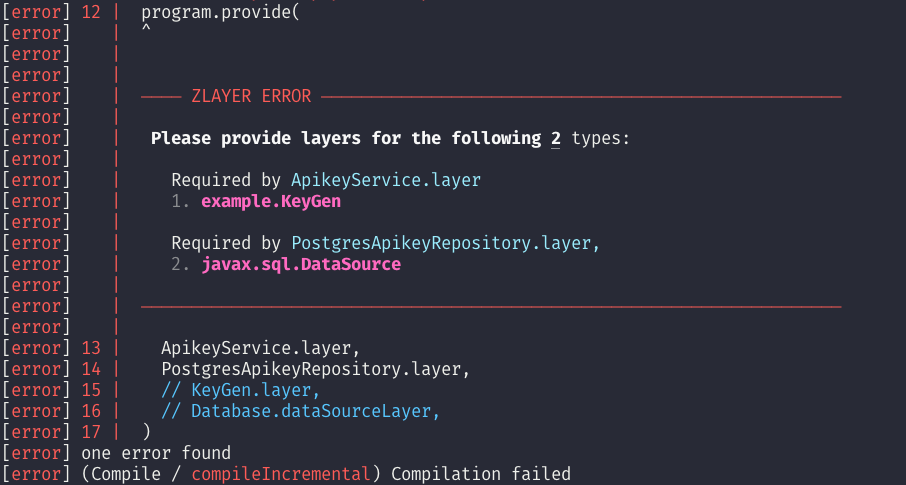
\includegraphics[width=\textwidth]{images/zlayer-provide-error.png}
    \caption{Error message produced by ZIO when required \inlinecode{ZLayer} is not provided.}
    \label{fig:zlayer-provide-error}
\end{figure}


\section{Testing}
The application contains several automated tests. ZIO has its own test library, zio-test, which was used for testing. There types of tests were written for the application: unit tests, integration tests and system tests. Unit tests run in-memory and exercise a single class or function. Integration tests ensure the correct functionality of multiple services together and may include out-of-process dependencies such as databases. Repository classes that interact with PostgreSQL database were tested with integration tests that used a database instance running in a Docker container. In system tests the application is tested as a whole, which in this case means that the configuration is read from environment variables and the database is running in a Docker container, similar to integration tests. System tests treat the application as a black box and tests only interact with its public API, which in this case is the HTTP endpoints.

Dependency injection in zio-test is managed \inlinecode{ZLayer}s. This makes it easy to configure the test in a way that the class under test can be provided with fake implementations of its dependencies. ZIO has also built-in \emph{test services} that make it possible to write deterministic tests that interact with console, time/clock, random generator and environment variables. This ability to effortlessly test interaction with time and environment variables in a controlled manner proved to be valuable.

\refsource{casestudy:testclock} shows a test for \inlinecode{ApikeyService} that verifies the revokation time of an API key is set to the current time. In the test a \inlinecode{TestClock} is used to fix the current time visible to the service, and then assert that the hardcoded time was actually used. The example also demonstrates how layers can be used to provide dependencies to the class under test.

\begin{algorithm}

\begin{minted}{scala}
test("revoke should set current time as the revokation time") {
  val fixedTime: Instant = Instant.parse("2023-03-30T19:34:28Z")

  for
    apikeyService <- ZIO.service[ApikeyService]
    apikey        <- apikeyService.create("test apikey description")

    _ <- TestClock.setTime(fixedTime) // Set current time
    _ <- apikeyService.revoke(apikey) // Perform logic under test

    // This is verifiable using the provided in-memory repository
    allApikeys    <- FakeApikeyRepository.getAll
    revokedApikey <- ZIO.getOrFail(allApikeys.find(_ == apikey))

  // Assert that the fixed time was used as the revokation time
  yield assertTrue(revokedApikey.isRevokedAt(fixedTime))
}.provide(
  ApikeyService.layer,
  FakeApikeyRepository.layer,
  FakeKeyGen.layer,
) // Test is configured with real ApikeyService and fake dependencies
\end{minted}

\caption{ZIO \inlinecode{TestClock} facilitates testing of code that uses the current time. \inlinecode{ZLayers} enable to inject desired dependencies to the service under test. \label{casestudy:testclock}}
\end{algorithm}

The biggest advantage of ZIO test services were however the possibility to configure the environment variables in system tests. The application reads its configuration, such as database connection string and HTTP port number, from environment variables. Traditionally testing how a program interacts with environment variables is cumbersome and error prone to say the least. ZIO \inlinecode{TestSystem} allows to set environment variables easily before the application is started and it tries to read its configuration. \refsource{casestudy:testsystem} shows a layer that requires environment variables that will be set before the application is started and kept running in the background.

\begin{algorithm}

\begin{minted}{scala}
case class EnvVars(values: Map[String, String])

object SystemTestSetup:
  // This layer starts the application in the background and
  // configures it by setting environment variables before starting.
  val layer: ZLayer[EnvVars, Nothing, Unit] =
    TestSystem.default >>> ZLayer.scoped {
      for
        envVars <- ZIO.service[EnvVars]
        _       <- setEnvironmentVariables(envVars)
        _       <- startApp
      yield ()
    }

  // The application keeps it running while tests are finished.
  // Delay makes sure the application has had time to start.
  def startApp = Main.run.forkScoped *> ZIO.sleep(2.second)

  def setEnvironmentVariables(envVars: EnvVars) =
    ZIO.foreachDiscard(envVars.values) { (key, value) =>
      TestSystem.putEnv(key, value)
    }
\end{minted}

\caption{ZIO \inlinecode{TestSystem} makes it possible to set/overwrite environment variables the application sees. This is used to set the configuration for the application in system tests. \label{casestudy:testsystem}}
\end{algorithm}

ZIO test services do not provide a way to control access to the file system, which is also quite hard to test because of similar reasons as environment variables. Even though the application in its current form does not use the file system, it would be nice if ZIO provided tools to test such interactions.


\section{Concurrency}
The application in its current form is quite simple, and thus ZIO's concurrency features were not needed much. This is probably partly due to the decision to use a relational database, which is able to perform complex query logic in a single query. In other projects there have been situations where it is necessary/beneficial to achieve concurrency when fetching data from multiple sources and combining the data in the application code. The situation is similar with NoSQL databases, which are usually not capable of doing joins in the database, thus forcing the joining logic to happen in the application code.

Other situations where ZIO's concurrency features could be useful is when the application has other functionalities besides just a HTTP interface. These other features could be scheduled batch jobs running in the background such as updating and invalidating caches or reporting metrics. Another common use case is asynchronous messaging where the application must listen to new messages in the background and react accordingly. ZIO's concurrency and scheduling capabilities are well suited for these kind of use cases.


\section{Analysis}
The case study revealed that using ZIO may initially slow down development, but this is only temporary and lasts for days or about one week. While the simplest tasks may sometimes be slightly more challenging to implement with ZIO, the benefits become apparent when dealing with more complex problems. The use of ZIO made it easier to tackle more difficult problems that may typically be ignored in imperative languages due to the time and effort required to solve them, such as examples in Listings \ref{casestudy:converterrors} and \ref{casestudy:retries} demonstrate. Some tasks that are unreasonably difficult (or even practically impossible) in mainstream languages are possible, often simple, with ZIO.

Acknowledging the ever changing and unpredictable nature of software projects, building new projects on strong foundations is desirable. This makes it possible to customize and evolve the software as effortlessly as possible. ZIO proved to be a robust foundation for developing applications that can confidently handle even the challenging problems. Refactoring is easy and could be done with confidence because ZIO programs are referentially transparent.

Developers with no previous experience with monadic effects or effects as values may find it difficult to comprehend programs written with ZIO. The programmer must be able to adopt a functional mindset in order to use ZIO (or other monadic effects) effectively.
    
\chapter{Conclusion}
\todo{Tästä luvusta puuttuu kommentit}

Monads are a way to encode effects that was discovered in the 90s. It is possible to use monads in a majority of current languages, as long as it has support for higher-order functions. Assuming used in a statically typed language, monads also provide an effect system, in addition to modeling effects. Monads have been used in the industry for a long time and it is quite mature method today. Challenges with monads is that they enforce that programs are written in monadic style. Also, combining different monadic effects is not straightforward and requires special treatment.

Algebraic effects and handlers are a more recent approach that was discovered in the early 2000s and first academic languages appearing in the 2010s. First languages with support for algebraic effects intended for commercial use surfaced in the early 2020s. In practice algebraic effects require a language that has native support for them. Such languages usually come with built-in effect system as well. These languages allow to write effectful programs in direct style, and combining different effects is effortless. However, algebraic effects and handlers are a recent practice with many open questions regarding how they should be included in the language.

Programming in a direct style with algebraic effects resembles imperative programming. It can be argued that the direct style of programming is more familiar to majority of programmers, thus making algebraic effects easier to comprehend than monadic effects. Monadic effects, on the other hand, are far more accessible to the average programmer than algebraic effects, since there are several monadic effect libraries available for different languages. Both methods enable highly expressive and modular effects; monads with combinators that modify a value representing a computation and algebraic effects with handlers that interpret the effect in a specific manner.

Capability based effects address many shortcomings with monads and algebraic effects. Their research is ongoing, and it is not yet possible to use them in practical applications, since languages with support for them are either academic or experimental. Nevertheless, proposals related to effect polymorphism and practical usability are promising.

Compared to unrestricted side effects, monads and algebraic effects provide attractive way to manage side effects, that differs from status quo. Controlling side effects with monads and algebraic effects is undeniably more expressive and compositional than unrestricted side effects. This is underlined by how convenient it is to implement re-usable logic for effects, such as retries and timeouts, with monads and algebraic effects compared to unrestricted side effects.

Programs written with monadic or algebraic effects have a tendency to be more declarative than their imperative counterparts with unrestricted side effects. These features facilitate the implementation of modular and resilient programs that are easier to modify and  which respond to errors in clearly defined manner. Concurrency concerns can be reduced, and high-level concurrency makes it easier to implement correct and performant programs when compared to working with traditional imperative low-level primitives, such as threads.

\todo{Pitääkö vielä tarkemmin jäsennellä ominaisuuksia tutkimuskysymyksiin peilaten?}

Algebraic effects with handlers and capability based solutions may eventually turn out to provide better developer ergonomics compared to monads, but currently there are little to none practical experience of using them in commercial software. It remains to be seen whether sophisticated methods for managing side effects will make their breakthrough in the industry. Eventually it's a matter of trade-off; are the sophisticated methods perceived useful enough to justify the initial education/learning required to comprehend them? In turn, is it possible to make these more sophisticated methods more accessible by making them feel more familiar to the average programmer, thus requiring less training? In the meantime, ZIO may well be one of the most compelling technologies to try out to get a taste of what these more advanced methods of handling side effects can offer today.

\todo{Lisää jotain case studysta}



% Hyvää pohdintaa ZIO:n heikkouksista: https://www.reddit.com/r/scala/comments/szmg95/error_tracking_is_commercially_worthless
% https://gist.github.com/djspiewak/741c60cff4959feb5272d88306595771 (Monads are Fundamental, Syntax is the Problem)
% Monads are a fundamental concept in modeling effectful computations as they define what sequential (the most natural and mandatory way of combining instructions) composition means
% The monadic syntax on the other hand might not be the solution for large scale adoption. Other library or language-level techniques like CPS-transformations, compiler/language macros and libraries utilizing these might make programming with effects attractive to masses.
% zio-direct, dotty-cps-async, Java Loom


\printbibliography

\begin{comment}
Important! Create the appendix chapters with command \textbackslash appchapter\{some
name\} instead of \textbackslash chapter\{some name\} for the automagic
page counting to work!
\end{comment}


\appchapter{Liitedokumentti}

Liitteen ohjelmakoodi kuvaa matemaattisen
monadirakenteen pohjalta rakentuvan Haskellin tyyppiluokan. Tyyppiluokan
voi nähdä eräänlaisena abstraktina ohjelmointirajapintana % (API\nomenclature[API]{API}{Application Programming Interface}),
joka muodostaa ohjelmoijalle abstraktin ohjelmointikielen käyttöliittymän
% (UI\nomenclature[UI]{UI}{User Interface}).

\end{document}
